\documentclass[11pt]{article}
\usepackage{cmap}
\usepackage[utf8]{inputenc}
\usepackage[T1]{fontenc}
\usepackage{amsmath,amssymb,amsthm}
\usepackage[hidelinks]{hyperref}
\usepackage{longtable}
\usepackage{array}
\usepackage{booktabs}
\usepackage{enumitem}
\usepackage{listings}
\usepackage{xcolor}
\usepackage{tikz}
\usepackage[margin=1.1in]{geometry}
\usepackage{fancyhdr}
\usepackage{graphicx}
\graphicspath{{figures/}}
\setlength{\emergencystretch}{2em}

% --- Lean 4 Syntax Highlighting ---
\lstdefinelanguage{lean4}{
  keywords={def, theorem, lemma, example, sorry, by, let, in, open, namespace,
            end, import, noncomputable, structure, instance, where, have, exact,
            apply, rw, simp, intro, constructor, linarith, nlinarith, ring_nf,
            field_simp, or_iff_right, mul_eq_zero},
  keywordstyle=\color{blue}\bfseries,
  ndkeywords={Real, Complex, Nat, Int, Set, Ioo, IsEssentiallySelfAdjoint, True, False},
  ndkeywordstyle=\color{purple}\bfseries,
  identifierstyle=\color{black},
  sensitive=true,
  comment=[l]{--},
  morecomment=[s]{/-}{-/},
  commentstyle=\color{gray}\itshape,
  stringstyle=\color{red},
  morestring=[b]",
  basicstyle=\ttfamily\small,
  breaklines=true,
  tabsize=2,
  captionpos=b,
  frame=single
}

% --- Draft Header/Footer ---
\pagestyle{fancy}
\fancyhf{}
\renewcommand{\headrulewidth}{0pt}
\fancyfoot[C]{\thepage}
\fancyfoot[R]{\footnotesize \textit{Academic Submission Draft. August 2026.}}

\title{Geometric Realization of Bicomplex Signal Manifolds:\\
       Spectral Stability, Whitney Folds, and Monodromy of the Observation Field}
\author{Akari Hayami (Jian-Yu Huang)}
\date{August 2026}

\DeclareMathOperator{\Ind}{Ind}
\newtheorem{theorem}{Theorem}[section]
\newtheorem{proposition}[theorem]{Proposition}
\newtheorem{lemma}[theorem]{Lemma}
\newtheorem{conjecture}[theorem]{Conjecture}
\newtheorem{corollary}[theorem]{Corollary}
\newtheorem{definition}[theorem]{Definition}
\newtheorem{remark}[theorem]{Remark}

\begin{document}
\maketitle

% --- Abstract ---
\begin{abstract}
We study a geometric framework for the realization of signal manifolds in
bicomplex space $\mathbb{C}^2$.  Starting from the momentum map
$\mu:\mathbb{C}^2\to\mathbb{R}^2$ and the power-conservation constraint
$|z_1|^2+|z_2|^2=1$, we derive a ruled-surface immersion $S(t,u)\in\mathbb{R}^3$
whose singularity structure is entirely governed by the quadratic invariant
$\mathcal{P}(c)=c^2-3c+1$, with unique root $c_0=\varphi^{-2}$ in $(0,1)$.

The paper separates intrinsic geometry from signal-theoretic and physical
observations.  The following results are proved rigorously.
\emph{(i)} Immersion singularities occur at exactly two lateral points $P_\pm$
where the complex observation field $F=N+iM$ carries topological indices
$\mathrm{Ind}(P_\pm)=\mp1$, with $|\det(DF)|_{P_\pm}|=5s_0(1-c_0)^2/Q_0$
(Theorem~\ref{thm:dipole_summary}, Corollary~\ref{cor:local_degree}).
\emph{(ii)} Any locally defined square root $\chi=\sqrt{F}$ acquires a sign
reversal after one loop around $P_+$, requiring $4\pi$ for geometric restoration
--- a monodromy result derived solely from the topological index
(Theorem~\ref{thm:monodromy}).
\emph{(iii)} The derivative of $\mathcal{P}$ at its root gives
$|\mathcal{P}'(c_0)|=\sqrt{5}$ exactly (Lemma~\ref{lem:sqrt5}).
\emph{(iv)} The Mellin dilation operator $\mathcal{T}_\sigma=-i(x\partial_x+\sigma)$
is formally self-adjoint iff $\sigma=\tfrac12$, with adjoint
$\mathcal{T}_\sigma^*=\mathcal{T}_{1-\sigma}$ derived by integration by parts
(Theorem~\ref{thm:formal_sa}).  When $T>2(M-1)/\delta$, the associated phasor
family is linearly independent with condition number
$\kappa(G)\le(1+\varepsilon)/(1-\varepsilon)$
(Proposition~\ref{prop:lin_indep}, Corollary~\ref{cor:condition_number}).
\emph{(v)} The fold and cross-cap normal forms have the intrinsic sublevel
exponent $3/4$; this yields a parameter-free logarithmic resolution law but not
a Shannon capacity formula.  \emph{(vi)} The normalization map of a cross-cap
produces a canonical constructible defect sheaf supported on its open double
locus.  \emph{(vii)} The Gram limit is the Haar orthogonality relation of the
Bohr torus, while $\sigma=\tfrac12$ is independently singled out by the
Dirichlet--Hardy evaluation boundary.  We also prove three scope limitations:
the proposed mass ratio retains a length scale, the natural sign-holonomy
boundary Dirac operator has vanishing APS $\eta$-invariant, and the constrained
source surface is not invariant under the full ambient $SU(2)$ action.
\emph{(viii)} After explicitly complexifying the cross-cap residual, its germ
is analytically equivalent to $X^2+Y^4$; its Milnor fiber is a twice-punctured
genus-one curve with monodromy spectrum $\{-i,1,i\}$ and Deligne weight-graded
dimensions $(2,1)$ in weights one and two.
\emph{(ix)} Every positive-radius link of the standard real cross-cap is a
circle whose image has one transverse double point and is therefore a
figure-eight graph.  Its normalization lift in $\mathbb R^4$ is embedded.  The
primitive weighted phase action of $X^2+Y^4$ has weights $(2,1)$ and produces
an embedded orbit in $\mathbb C^2$ whose rectangular shadow is a transverse
Lissajous figure-eight with exact dimensionless frequency ratio $2:1$.
\emph{(x)} For the actual lateral ruled-surface germs $P_\pm$, the three
canonical Whitney two-jet invariants $(a_\pm,b_\pm,c_\pm)$ satisfy
$b_\pm^2+a_\pm c_\pm^2=0$.  Hence the normal-plane trace of the associated
principal-curvature surface is a cusp rather than a transverse figure-eight;
this closes that direct geometric bridge.

The repeated appearances of $\sqrt5$, the $4\pi$ restoration, and the
half-density line remain noteworthy signal or physical analogies.  They are
reported as observations rather than as established capacity, particle-mass,
chirality, or Weil-cohomological identifications.  The Deligne structure just
stated belongs only to the explicitly chosen complex residual fiber; it is not
inferred from $\sigma=1/2$ or from the real signal geometry alone.
\end{abstract}

% --- Introduction ---
\section{Introduction}
This study investigates a geometric model connecting signal physics and
singularity theory using the tools of classical differential geometry.
We define a signal manifold $\mathcal{S} \subset \mathbb{C}^2$ and an associated
operator space $\mathcal{H}_S \cong L^2([1, \infty), dx)$ equipped with a
weighted Hilbert metric:
\[
  \langle f, g \rangle_{\sigma}
  = \int_1^\infty f(x)\,\overline{g(x)}\,x^{2\sigma-1}\,dx.
\]
Two singular structures must be distinguished.  Rank loss of
$S:D\to\mathbb R^3$ produces cross-cap germs, whereas the planar observation
map $\Psi=(N,M):D\to\mathbb R^2$ has fold behaviour.  We show that the
topological dipole of $F=N+iM$ implies a $4\pi$ monodromy
(Section~\ref{sec:mono}), and that the formal-adjoint threshold of the associated
dilation operator occurs at $\sigma = \tfrac12$ (Section~\ref{sec:spectral}).
Section~\ref{sec:condensed} replaces earlier condensed/Weil analogies by
constructible-sheaf, Hardy--Dirichlet, and Bohr--Haar statements with explicit
scope limits.  The same audit now separates the real cross-cap residual from
its explicitly chosen complex algebraic completion, for which Milnor
monodromy and Deligne weights can be computed.  The same completion also
supplies a primitive $(2,1)$ phase lift: its smooth four-real-dimensional orbit
projects to a planar figure-eight, while one restored phase coordinate gives an
exact reconstruction.  A separate two-jet calculation for the actual lateral
ruled-surface cross-caps shows that their principal-curvature exceptional
traces remain cusps and therefore do not identify either figure-eight
construction.  Signal and physical
similarities are retained as noteworthy
observations, never as substitutes for missing operators or dynamics.

% --- Preliminaries ---
\section{Preliminaries}
\subsection{Bicomplex Space and Unitary Modulations}
Let $\mathbb{C}^2 \cong \mathbb{R}^4$.  A signal state
$\mathbf{z} = (z_1, z_2)^\top$ under the total power constraint
$|z_1|^2 + |z_2|^2 = 1$ defines a 3-sphere $S^3$.  Unitary signal modulations
correspond to $SU(2)$ operations on this ambient space.  The constrained
two-dimensional source used below is a proper subset of $S^3$ and is not itself
invariant under the full transitive left action of $SU(2)$;
Proposition~\ref{prop:su2_scope} makes this distinction precise.

\subsection{Whitney Fold Singularities}
A smooth mapping $f: \mathbb{R}^n \to \mathbb{R}^m$ has a \emph{fold singularity}
at a point if it is locally equivalent to the normal form
$(\xi, \eta) \mapsto (\xi, \eta^2)$ \cite{GolubitskiGuillemin1973, Whitney1955, Arnold1991}.
In the context of 4D-to-3D projections, this singularity generates a
double-sheeted covering of the observational plane, where the two sheets
represent distinct internal phases of the same observable coordinate.

\begin{figure}[htbp]
\centering
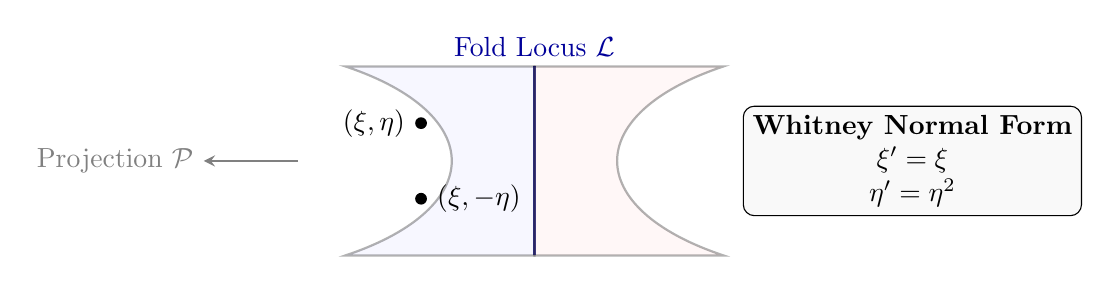
\begin{tikzpicture}[scale=1.2, >=stealth]
  \draw[thick, blue!60!black] (0,-1) -- (0,1) node[above] {Fold Locus $\mathcal{L}$};
  \draw[thick, opacity=0.3, fill=blue!10] (-2,-1) .. controls (-0.5,-0.5) and
    (-0.5,0.5) .. (-2,1) -- (0,1) -- (0,-1) -- cycle;
  \draw[thick, opacity=0.3, fill=red!10] (2,-1) .. controls (0.5,-0.5) and
    (0.5,0.5) .. (2,1) -- (0,1) -- (0,-1) -- cycle;
  \node[circle, fill=black, inner sep=1.5pt, label=left:{$(\xi, \eta)$}]
    (p1) at (-1.2, 0.4) {};
  \node[circle, fill=black, inner sep=1.5pt, label=right:{$(\xi, -\eta)$}]
    (p2) at (-1.2, -0.4) {};
  \draw[->, thick, gray] (-2.5, 0) -- (-3.5, 0)
    node[left] {Projection $\mathcal{P}$};
  \node[draw, rounded corners, fill=gray!5, align=center] at (4.0, 0) {
    \textbf{Whitney Normal Form} \\
    $\xi' = \xi$ \\
    $\eta' = \eta^2$
  };
\end{tikzpicture}
\caption{Schematic of a Whitney fold singularity.  The mapping collapses two
  sheets onto a single observational plane, creating a $2:1$ covering.}
\label{fig:whitney_fold}
\end{figure}

% --- Definitions ---
\section{Formal Definitions}
\label{sec:defs}

\subsection{The Bicomplex Signal Manifold}
The Bicomplex Signal Manifold $\mathcal{S}$ is derived from the constraint
$|z_1|^2 + |z_2|^2 = 1$ via the momentum map $\mu: \mathbb{C}^2 \to \mathbb{R}^2$,
$\mu(\mathbf{z}) = (|z_1|^2, |z_2|^2) = (X, Y)$.  Setting $X = c := \cos t$ and
$Y = 1-c = \cos\phi$, the constraint $\cos t + \cos\phi = 1$ parametrizes a
family of ruling lines.  With $Q(t) = \sqrt{2c - c^2}$ and ruling parameter
$u \in [0,1]$, the immersion is
\begin{equation}\label{eq:immersion}
  S(t,u)
  = (c + 2u(1-c),\; (1-u)s,\; uQ)^\top, \qquad s = \sin t,
\end{equation}
a non-developable ruled surface studied in detail in \cite{HayamiRuledSurface2026};
basic differential-geometric notation follows \cite{doCarmo1976}.

\begin{definition}[Geometric Projection]
The \emph{Geometric Projection} $\mathcal{P}: \mathbb{R}^4 \to \mathbb{R}^3$
maps the 4D signal state to 3D observational space.  The realization
$\mathcal{P}(\mathcal{S})$ exhibits immersion singularities where the normal
vector $V = S_t \times S_u$ vanishes.
\end{definition}

\begin{definition}[Mellin--Hilbert Spectral Operator]
\label{def:mellin_hilbert}
The \emph{Mellin--Hilbert Spectral Operator} is the family of operators
\[
  \mathcal{T}_\sigma = -i\!\left(x\,\frac{d}{dx} + \sigma\right),
  \qquad \sigma \in \mathbb{R},
\]
acting on $\mathcal{D} = C_c^\infty((1,\infty)) \subset L^2([1,\infty), dx)$.
The formal eigenfunctions $f_\omega(x) = x^{-(\sigma + i\omega)}$ satisfy
$\mathcal{T}_\sigma f_\omega = -\omega\, f_\omega$ with \emph{real} eigenvalue
$-\omega$ (see Corollary~\ref{cor:real_eigvals}).
\end{definition}

\begin{definition}[Singular Resolution Cost]
For a non-negative local residual $K$ and $\varepsilon>0$, define
\[
  V_K(\varepsilon):=\operatorname{vol}\{x:K(x)\le\varepsilon\},
  \qquad
  \mathcal C_K(\varepsilon):=-\log V_K(\varepsilon).
\]
This is a geometric resolution cost.  It is not called a communication-channel
capacity unless a probability law, noise model, and resource constraint are
specified independently.
\end{definition}

% --- Geometric Monodromy ---
\section{Geometric Monodromy of the Observation Field}
\label{sec:mono}
The cross product $V = S_t \times S_u$ yields the complex observation field
$F := N + iM$ where $N = V_z$ and $M = V_x$.  The following summarises results
from \cite{HayamiRuledSurface2026}.

\begin{theorem}[Topological Dipole \cite{HayamiRuledSurface2026}]
\label{thm:dipole_summary}
The field $F = N + iM$ has exactly two isolated zeros
$P_\pm = (\pm t_0, u_0)$ with indices $\Ind(P_+) = -1$ and $\Ind(P_-) = +1$.
At $P_+$ the Jacobian determinant of $(t,u)\mapsto(N,M)$ equals
$-5s_0(1-c_0)^2/Q_0 < 0$, confirming non-degeneracy.
\end{theorem}

\begin{theorem}[Geometric Monodromy and $4\pi$ Restoration]
\label{thm:monodromy}
Let $\gamma: [0,1] \to U \setminus \{P_+\}$ be a small positively oriented loop
encircling $P_+$ once.  Any locally defined square root $\chi = \sqrt{F}$ along
$\gamma$ satisfies
\[
  \chi(\gamma(1)) = -\chi(\gamma(0)).
\]
Consequently the geometric period of $\chi$ in parameter space is $4\pi$: two
full traversals of $\gamma$ are required to restore $\chi$.
\end{theorem}

\begin{proof}
By Theorem~\ref{thm:dipole_summary}, $\Ind(P_+) = -1$, meaning the winding number
of $F \circ \gamma$ around the origin in $\mathbb{C}$ equals $-1$.  Write
$F(\gamma(s)) = R(s)\,e^{i\alpha(s)}$ for a continuous argument $\alpha$.
Since the winding number is $-1$, we have $\alpha(1) = \alpha(0) - 2\pi$.

Define the square root branch $\chi(\gamma(s)) = \sqrt{R(s)}\,e^{i\alpha(s)/2}$.
At $s = 1$:
\begin{align*}
  \chi(\gamma(1))
  &= \sqrt{R(0)}\,e^{i(\alpha(0)-2\pi)/2}\\
  &= \sqrt{R(0)}\,e^{i\alpha(0)/2}\cdot e^{-i\pi}\\
  &= -\chi(\gamma(0)).
\end{align*}
After a second traversal, $\alpha(2) = \alpha(0) - 4\pi$, giving
$\chi(\gamma(2)) = \sqrt{R(0)}\,e^{i(\alpha(0)-4\pi)/2} = +\chi(\gamma(0))$.
Thus $4\pi$ is the minimal period.

The sign flip $\chi \to -\chi$ corresponds geometrically to a transition
between the two sheets of the Whitney double cover along the fold locus
$\mathcal{L}$: the two preimages $(\xi_0, +\sqrt{\varepsilon})$ and
$(\xi_0, -\sqrt{\varepsilon})$ (Whitney normal form, \cite{GolubitskiGuillemin1973})
differ in the sign of the transversal coordinate $\eta$, and the observational
Jacobian $J = 2\eta$ changes sign accordingly.
\end{proof}

\begin{remark}
Theorem~\ref{thm:monodromy} establishes a purely geometric monodromy result:
the complex field $F$, whose topological dipole structure is rigorously derived
from the surface geometry, forces any branch of $\sqrt{F}$ to have period $4\pi$.
This is \emph{analogous} to spinor periodicity in $SU(2)$, but the identification
with physical Spin-$\tfrac12$ requires additional physical assumptions and is not
claimed here as a mathematical theorem.
\end{remark}

\begin{corollary}[Local Degree via Jacobian Sign]
\label{cor:local_degree}
For a smooth map $\Phi: \mathbb{R}^2 \to \mathbb{R}^2$ with an isolated zero at
$p$ and non-degenerate Jacobian $\det(D\Phi(p)) \neq 0$, the topological index
satisfies
\[
  \mathrm{Ind}(p) = \mathrm{sgn}\bigl(\det(D\Phi(p))\bigr).
\]
Applied to $\Phi = (N,M)$ and the lateral singularities:
\begin{align*}
  \det(DF)\big|_{P_+}
  &= -\frac{5\,s_0(1-c_0)^2}{Q_0} < 0
  \;\Rightarrow\; \mathrm{Ind}(P_+) = -1, \\
  \det(DF)\big|_{P_-}
  &= +\frac{5\,s_0(1-c_0)^2}{Q_0} > 0
  \;\Rightarrow\; \mathrm{Ind}(P_-) = +1.
\end{align*}
This gives an explicit, computable derivation of the topological dipole, with
numerical values $|\det(DF)|_{P_\pm}| \approx 2.245$.
\end{corollary}

\begin{proof}
The local degree formula $\mathrm{Ind}(p) = \mathrm{sgn}(\det D\Phi(p))$ is
standard for non-degenerate zeros of smooth planar maps \cite{GolubitskiGuillemin1973}.
The Jacobian values are computed in \cite{HayamiRuledSurface2026} (Theorem~4.1)
from the explicit formulae $N_u, N_t, M_u, M_t$ at $(c_0, u_0)$
using $c_0^2 = 3c_0 - 1$.  The parity identity
$\det(DF)|_{P_-} = -\det(DF)|_{P_+}$ follows from $N,M$ being even/odd functions
of $t$ respectively, so the sign flips under $t_0 \mapsto -t_0$.
\end{proof}

\begin{figure}[htbp]
\centering
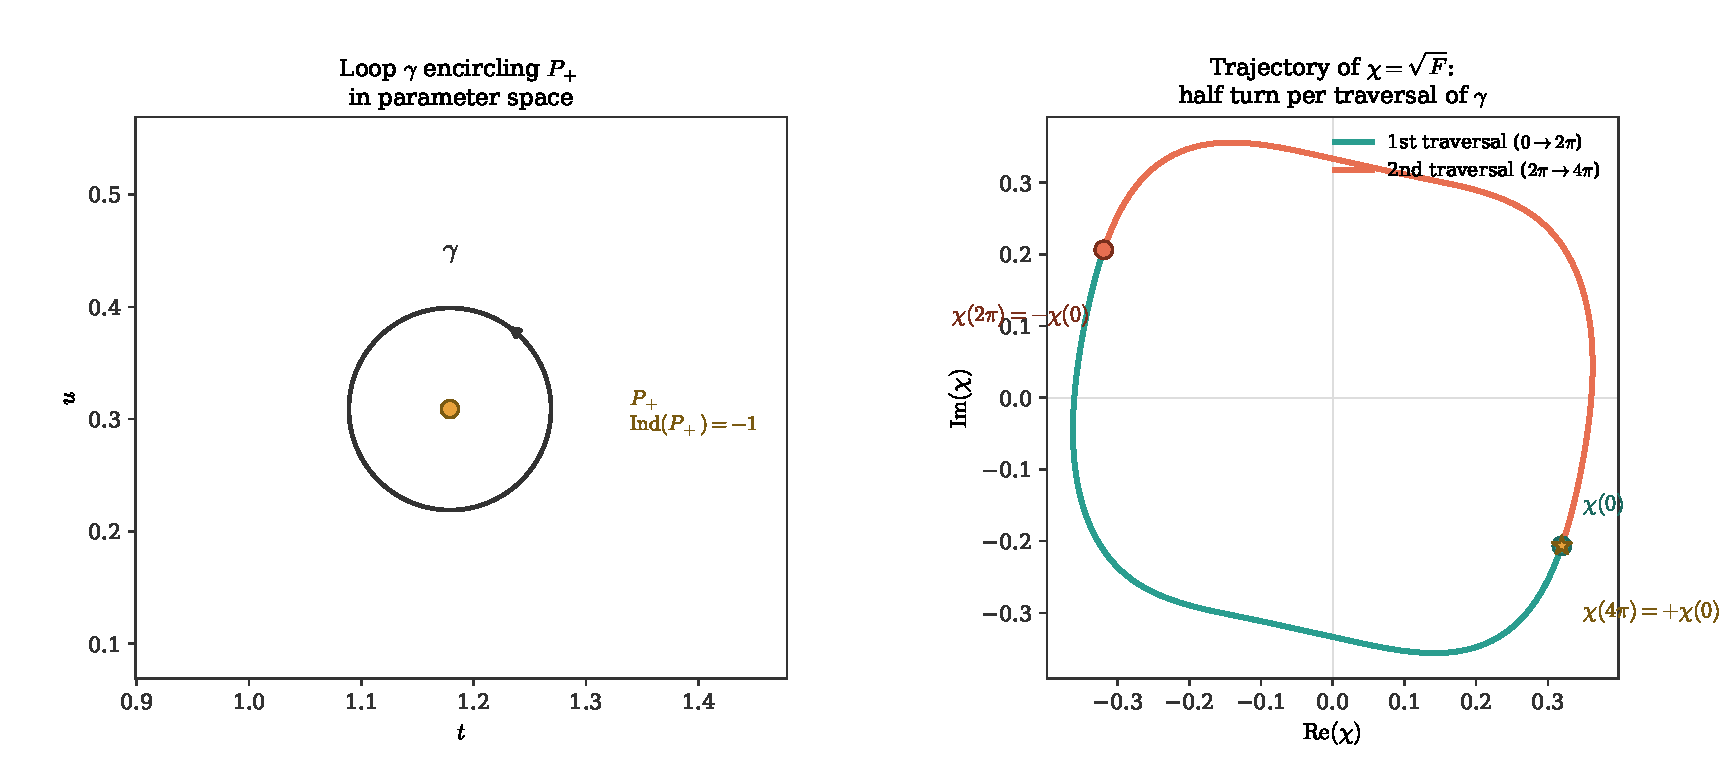
\includegraphics[width=0.85\textwidth]{fig6_monodromy_loop.pdf}
\caption{Geometric monodromy of $\chi=\sqrt{F}$ (Theorem~\ref{thm:monodromy}).
  Left: a positively oriented loop $\gamma$ encircling $P_+$ in parameter
  space; $\mathrm{Ind}(P_+)=-1$.  Right: the resulting trajectory of $\chi$
  in $\mathbb{C}$.  Because the index is $-1$, the argument of $\chi$ advances at
  half the rate of $\gamma$'s winding, so one traversal (teal) sweeps only
  half a turn, from $\chi(0)$ to the antipodal point $\chi(2\pi)=-\chi(0)$; a
  second traversal (coral) is required to close the loop, giving the minimal
  geometric period $4\pi$.}
\label{fig:monodromy_loop}
\end{figure}

% --- Intrinsic singular scaling ---
\section{Intrinsic Singular Compression at the Anchor}
\label{sec:scaling}
We first retain the exact derivative attached to the normalized invariant
polynomial, then derive a coordinate-invariant local scaling exponent from the
singularity normal form.

\begin{lemma}[Spectral Compression Rate]
\label{lem:sqrt5}
The derivative of the core invariant polynomial $\mathcal{P}(c) = c^2 - 3c + 1$
at its root $c_0 = (3-\sqrt{5})/2$ satisfies
\[
  |\mathcal{P}'(c_0)| = \sqrt{5}.
\]
\end{lemma}

\begin{proof}
$\mathcal{P}'(c) = 2c - 3$.  At $c_0 = (3-\sqrt{5})/2$:
\[
  \mathcal{P}'(c_0)
  = 2\cdot\frac{3-\sqrt{5}}{2} - 3
  = (3-\sqrt{5}) - 3
  = -\sqrt{5}.
\]
Hence $|\mathcal{P}'(c_0)| = \sqrt{5}$. \qed
\end{proof}

\begin{remark}
The Jacobian determinant at $P_+$ evaluated in \cite{HayamiRuledSurface2026} is
$5s_0(1-c_0)^2/Q_0 \approx 2.245$, which is numerically close to but not exactly
$\sqrt{5} \approx 2.236$.  The exact value involves
$(1-c_0) = \varphi^{-1}$, $Q_0 = \varphi^{-1/2}$, and
$s_0 = \sqrt{(3\sqrt{5}-5)/2}$.
Lemma~\ref{lem:sqrt5} identifies $\sqrt{5}$ as the rate of vanishing of the
\emph{chosen monic polynomial} $\mathcal P$.  It is not an invariant of the zero
germ by itself: replacing $\mathcal P$ by $a\mathcal P$, $a\ne0$, preserves the
zero set but changes the derivative to $|a|\sqrt5$.  The
same constant reappears as an intensity, rather than a rate: in the
companion paper~\cite{HayamiStokesCaustic2026}, the Stokes caustic on the
Poincar\'{e} sphere induced by the fold locus of $\mathcal{S}$ has total
intensity exactly $\sqrt5/2=|\mathcal{P}'(c_0)|/2$ at its far endpoint---an
independent derivation converging on the same constant.  This repetition is a
noteworthy structural observation, but it does not by itself define capacity.
\end{remark}

\begin{theorem}[Intrinsic Sublevel Exponent]
\label{thm:sublevel_exponent}
For the Whitney fold $f_{\mathrm f}(x,y)=(x,y^2)$ with squared residual
$K_{\mathrm f}=\|f_{\mathrm f}\|^2=x^2+y^4$,
\[
  V_{K_{\mathrm f}}(\varepsilon)
  =\mathrm B\!\left(\tfrac14,\tfrac32\right)\varepsilon^{3/4}.
\]
For the Whitney cross-cap $f_\times(x,y)=(x,xy,y^2)$ with
$K_\times=\|f_\times\|^2=x^2(1+y^2)+y^4$,
\[
  V_{K_\times}(\varepsilon)
  =\mathrm B\!\left(\tfrac14,\tfrac32\right)
   \varepsilon^{3/4}\bigl(1+o(1)\bigr).
\]
Thus both local models have the intrinsic sublevel, or singular-learning,
exponent $\lambda=3/4$.
\end{theorem}

\begin{proof}
For the fold,
\begin{align*}
V_{K_{\mathrm f}}(\varepsilon)
 &=4\int_0^{\varepsilon^{1/4}}\sqrt{\varepsilon-y^4}\,dy\\
 &=4\varepsilon^{3/4}\int_0^1\sqrt{1-t^4}\,dt
 =\mathrm B\!\left(\tfrac14,\tfrac32\right)\varepsilon^{3/4}.
\end{align*}
For the cross-cap, set $x=\varepsilon^{1/2}s$ and
$y=\varepsilon^{1/4}t$.  The Jacobian is $\varepsilon^{3/4}$ and the rescaled
sublevel condition is
$s^2(1+\varepsilon^{1/2}t^2)+t^4\le1$, which converges to
$s^2+t^4\le1$.  Dominated convergence gives the stated constant and exponent.
This agrees with the metric interpretation of real log-canonical thresholds by
sublevel-volume asymptotics \cite{Grulha2026}.
\end{proof}

\begin{remark}[A Logarithmic Signal-Resolution Observation]
If an operational model independently identifies $S=\varepsilon^{-1}$, then
Theorem~\ref{thm:sublevel_exponent} gives
\[
  \mathcal C_K(S^{-1})=\tfrac34\log S
  -\log\mathrm B\!\left(\tfrac14,\tfrac32\right)+o(1).
\]
It is worth noting that a logarithmic law survives, but its intrinsic local
coefficient is $3/4$, not $\sqrt5$.  Calling this quantity a Shannon capacity
would still require a channel law and a noise/resource constraint; no such
physical identification is asserted here.
\end{remark}

\begin{proposition}[Residual Geometry Does Not Fix Channel Capacity]
\label{prop:capacity_nogo}
The residual germ and its sublevel volumes do not uniquely determine a Shannon
capacity.
\end{proposition}

\begin{proof}
On fixed binary input and output alphabets, the constant channel
$P(Y=0\mid X=0)=P(Y=0\mid X=1)=1$ has capacity zero, whereas the noiseless
channel $P(Y=X\mid X)=1$ has capacity $\log 2$.  The source and observation
labels may be held fixed while the stochastic kernel changes.  Since the
residual germ supplies no kernel, input constraint, or noise scale, it cannot
select between these values.
\end{proof}

\subsection{Complex Analytic Completion of the Cross-Cap Residual}

The following completion is made only after extending the coefficients of
$K_\times$ from $\mathbb R$ to $\mathbb C$.  This is explicit algebraic input,
not a reconstruction from the real image topology.

\begin{theorem}[$A_3$ residual germ]
\label{thm:a3_residual}
The complex analytic germ
\[
 K_\times(x,y)=x^2(1+y^2)+y^4
\]
is right-equivalent at the origin to $f(X,Y)=X^2+Y^4$.  Its Milnor and
Tjurina numbers are $\mu(K_\times)=\tau(K_\times)=3$.
\end{theorem}

\begin{proof}
On a small disk about $y=0$, choose the holomorphic branch
$u(y)=(1+y^2)^{1/2}$ with $u(0)=1$, and set $X=xu(y)$, $Y=y$.
The Jacobian determinant at the origin is one, so this is a local
biholomorphism, and $K_\times=X^2+Y^4$.  Its Jacobian algebra is
\[
 \frac{\mathbb C\{X,Y\}}{(2X,4Y^3)}
 \cong\frac{\mathbb C\{Y\}}{(Y^3)},
\]
with basis $1,Y,Y^2$.  Weighted homogeneity gives
$f=\tfrac12X\partial_Xf+\tfrac14Y\partial_Yf$, so $f$ lies in the Jacobian
ideal and the Tjurina algebra has the same dimension.
\end{proof}

\begin{theorem}[Milnor fiber and finite monodromy]
\label{thm:a3_milnor}
The global Milnor fiber
\[
 U=\{(X,Y)\in\mathbb C^2:X^2+Y^4=1\}
\]
is a genus-one curve with two points removed.  Hence
$\dim H^1(U;\mathbb Q)=3$.  Its geometric monodromy can be chosen as
\[
 h(X,Y)=(-X,iY),\qquad h^4=\mathrm{id},
\]
and on first cohomology
\[
 \operatorname{spec}(h^*)=\{-i,1,i\},\qquad
 \det(tI-h^*)=(t-1)(t^2+1).
\]
\end{theorem}

\begin{proof}
Weighted homogeneity identifies $U$ with the local Milnor fiber
\cite{Milnor1968,Dimca1992}.  Compactify it as
\[
 E:\quad X^2+Y^4=Z^4\subset\mathbb P(2,1,1).
\]
Projection to $[Y:Z]\in\mathbb P^1$ is a double cover branched at four
simple points.  Riemann--Hurwitz gives $g(E)=1$.  The fiber above
$[Y:Z]=[1:0]$ contains two unramified points, so $U=E\setminus D$ with
$|D|=2$ and $b_1(U)=2g(E)+|D|-1=3$.

The displayed $h$ is the weighted-homogeneous monodromy.  The differential
$\omega=dY/X$ spans $H^{1,0}(E)$ and satisfies $h^*\omega=-i\omega$; its
conjugate has eigenvalue $i$.  With $s=1/Y$ and $W=X/Y^2$ near infinity,
$h(s,W)=(-is,W)$, so both points of $D$ and the logarithmic boundary class are
fixed.  These three classes exhaust $H^1(U;\mathbb C)$.
\end{proof}

\subsection{Figure-Eight Links and the Weighted Phase Lift}

The real cross-cap and its chosen $A_3$ completion carry two related, but
distinct, figure-eight constructions.  The first is the link of the real
cross-cap image.  The second is a planar shadow of the weighted phase orbit in
$\mathbb C^2$.  Keeping them separate prevents a projected self-intersection
from being mistaken for a singularity of the lifted source.

\begin{proposition}[The cross-cap link is a figure-eight quotient]
\label{prop:crosscap_figure_eight}
For $r>0$, let
\[
 L_r:=\{(x,y)\in\mathbb R^2:K_\times(x,y)=r^2\}.
\]
Then $L_r$ is a smooth circle.  The restriction
$f_\times|_{L_r}:L_r\to S_r^2$ is an immersion with exactly one transverse
double point,
\[
 f_\times(0,\sqrt r)=f_\times(0,-\sqrt r)=(0,0,r).
\]
Consequently its image is homeomorphic to the figure-eight graph
$S^1\vee S^1$.  Moreover,
\[
 \widetilde f_\times(x,y):=(x,xy,y^2,y)\in\mathbb R^4
\]
is an embedding and satisfies the reconstruction identity
\[
 \pi_{123}\circ\widetilde f_\times=f_\times,
\]
where $\pi_{123}$ forgets the last coordinate.
\end{proposition}

\begin{proof}
The gradient
\[
 \nabla K_\times
 =\bigl(2x(1+y^2),\,2x^2y+4y^3\bigr)
\]
vanishes only at the origin, which is not in $L_r$.  Thus $L_r$ is a smooth
compact one-manifold.  It is connected because it is the union of the two
graphs
\[
 x=\pm\sqrt{\frac{r^2-y^4}{1+y^2}},
 \qquad -\sqrt r\le y\le\sqrt r,
\]
joined at their two endpoints; hence $L_r\cong S^1$.

If $f_\times(x,y)=f_\times(x',y')$, then $x=x'$ and $y'^2=y^2$.
The case $y'=y$ gives the same source point.  If $y'=-y$, equality of the
second coordinates gives $xy=-xy$.  The only distinct pair on $L_r$ is
therefore $(0,\sqrt r)$ and $(0,-\sqrt r)$.  At these points the source
tangent is spanned by $(1,0)$, and its two image tangents are
\[
 (1,\sqrt r,0),\qquad (1,-\sqrt r,0).
\]
Their cross product is $(0,0,-2\sqrt r)\ne0$, so the double point is
transverse.  Identifying exactly two distinct points of a circle gives
$S^1\vee S^1$.  Finally, the first and fourth coordinates of
$\widetilde f_\times$ recover $(x,y)$, so it is an embedding, and the displayed
projection identity is immediate.
\end{proof}

\begin{theorem}[$A_3$ weighted phase orbit and figure-eight shadow]
\label{thm:a3_weighted_figure_eight}
The primitive positive integral weights of $X^2+Y^4$ are $(2,1)$.  Define
\[
 \Phi_s(X,Y):=(e^{2is}X,e^{is}Y).
\]
Then
\[
 f(\Phi_s(X,Y))=e^{4is}f(X,Y),
 \qquad \Phi_{\pi/2}=h.
\]
For any $a,b>0$ satisfying $a^2+b^4=1$, the orbit
\[
 \Gamma_{a,b}(s):=(ae^{2is},be^{is}),
 \qquad s\in\mathbb R/2\pi\mathbb Z,
 \label{eq:a3_weighted_orbit}
\]
is an embedded circle in $\mathbb C^2$.  Its rectangular projection
\[
 P(\Gamma_{a,b}(s))=(\operatorname{Im}Y,\operatorname{Im}X)
 =(b\sin s,a\sin2s)
 \label{eq:a3_figure_eight_projection}
\]
has exactly one transverse double point and obeys
\[
 v^2=4a^2\frac{u^2}{b^2}
 \left(1-\frac{u^2}{b^2}\right).
 \label{eq:a3_figure_eight_equation}
\]
Adding the single lost coordinate $\operatorname{Re}Y=b\cos s$ reconstructs
the lifted orbit.  Along the phase parameter,
\[
 \frac{d^2X}{ds^2}+4X=0,
 \qquad
 \frac{d^2Y}{ds^2}+Y=0,
\]
so the dimensionless frequency ratio is exactly $2:1$.
\end{theorem}

\begin{proof}
Weighted homogeneity requires $2w_X=4w_Y$; primitivity therefore gives
$(w_X,w_Y)=(2,1)$.  Direct substitution proves the covariance formula, and
$s=\pi/2$ gives $(-X,iY)=h(X,Y)$.  Since $b>0$, the $Y$ coordinate determines
$s$ modulo $2\pi$, so $\Gamma_{a,b}$ is embedded.

Set $u=b\sin s$ and $v=a\sin2s$.  Eliminating $s$ gives
Equation~\eqref{eq:a3_figure_eight_equation}.  If two parameter values have
the same $(u,v)$, the only distinct pair is $s=0,\pi$.  Their projected
tangents are $(b,2a)$ and $(-b,2a)$, whose determinant is $4ab\ne0$.
The pair $(\operatorname{Re}Y,\operatorname{Im}Y)$ recovers $be^{is}$ and
hence $s$, after which $X=ae^{2is}$ is fixed.  The oscillator equations follow
by differentiating Equation~\eqref{eq:a3_weighted_orbit} twice.
\end{proof}

\begin{proposition}[The Euclidean phase action does not fix the bridge]
\label{prop:a3_amplitude_nogo}
For the orbit family in Theorem~\ref{thm:a3_weighted_figure_eight}, the
Euclidean quadratic action is
\[
 \mathcal E(a,b)
 :=\int_0^{2\pi}\|\Gamma'_{a,b}(s)\|^2\,ds
 =2\pi(4a^2+b^2).
\]
Subject to $a^2+b^4=1$, its minimum is the degenerate orbit $(a,b)=(0,1)$.
Its unique interior critical point satisfies
\[
 b^2=\frac18,
 \qquad a^2=\frac{63}{64},
\]
and is a strict maximum.  Thus this action fixes neither a non-degenerate
figure-eight amplitude nor an absolute clock.
\end{proposition}

\begin{proof}
Put $z=b^2\in[0,1]$.  The constraint gives $a^2=1-z^2$, and hence
\[
 \frac{\mathcal E}{2\pi}=4+z-4z^2.
\]
This polynomial is strictly concave.  Its minimum occurs at the endpoint
$z=1$, where $a=0$, while its only interior critical point $z=1/8$ is the
strict maximum.  Replacing $s$ by $\omega_0t$ leaves the ratio $2:1$ unchanged
for every $\omega_0>0$, so the geometry supplies no absolute time scale.
\end{proof}

\begin{remark}[Wave and reconstruction scope]
The phase orbit gives an exact two-frequency oscillator, not yet a spacetime
wave equation.  Treating its planar shadow as a metric graph would require an
independent matching condition at the four-valent vertex
\cite{EngelKramar2019}.  The normalization lift instead keeps the two source
points distinct and therefore specifies source continuation without creating
a physical scattering vertex.  The value $b^4=1/64$ at the interior maximum
of Proposition~\ref{prop:a3_amplitude_nogo} is metric- and action-dependent;
it is not identified with $1/(64\pi^2)$.
\end{remark}

\begin{proposition}[The actual ruled cross-caps remain on the cusp boundary]
\label{prop:actual_principal_cusp}
Let $P_\sigma=(\sigma t_0,u_0)$, $\sigma\in\{+1,-1\}$, be the two lateral
cross-caps of the ruled surface $S$, and write its unique oriented Euclidean
Whitney normal form as in \cite[Proposition~2.1]{MartinsEtAl2026}.  Its
second-order invariants $(a_\sigma,b_\sigma,c_\sigma)$ are
\begin{align*}
 a_\sigma&=-\frac{M^2}{2N^{3/2}},
 &b_\sigma&=\sigma\frac{\sqrt{M^2R}}{N},
 &c_\sigma&=\frac{\sqrt{2R}}{N^{1/4}},\\
 N&=\frac{-335+162\sqrt5}{12},
 &M^2&=\frac{-520+249\sqrt5}{27},
 &R&=\frac{20(140+11\sqrt5)}{11397}.
\end{align*}
In particular,
\[
 (a_+,b_+,c_+)\approx(-0.1991214663,0.2763032014,0.6191941949),
\]
while $a_-=a_+$, $b_-=-b_+$, and $c_-=c_+$.  The orientation-free data are
$a_\sigma$, $|b_\sigma|$, and $c_\sigma$.  They obey the exact identity
\begin{equation}
 b_\sigma^2+a_\sigma c_\sigma^2=0.
 \label{eq:actual_principal_cusp_identity}
\end{equation}
Consequently the polynomial selecting returns of the principal-curvature
exceptional trace to the origin factors as
\[
 c_\sigma\tau^2+2b_\sigma\tau-a_\sigma c_\sigma
 =c_\sigma\left(\tau+\frac{b_\sigma}{c_\sigma}\right)^2.
\]
The trace therefore has a double return direction and a cusp, not a
transverse node or figure-eight.
\end{proposition}

\begin{proof}
Put $c_0=(3-\sqrt5)/2$, $u_0=(\sqrt5-1)/4$, and
$s_\sigma=\sigma\sqrt{2-3c_0}$.  At $P_\sigma$ choose the adapted pair
\[
 \xi_0=\frac1{\sqrt3}\partial_u,
 \qquad
 \eta_0=-\partial_t+\lambda_\sigma\partial_u,
 \qquad
 \lambda_\sigma=-\frac{c_0s_\sigma}{2(1-c_0)}.
\]
Let $\Pi_N$ be orthogonal projection onto the normal plane of the rank-one
image and set
\[
 A=\Pi_N(S_{tt}-2\lambda_\sigma S_{tu}),
 \qquad B=\Pi_N(-S_{tu}/\sqrt3).
\]
Direct substitution into the ruled-surface derivatives gives
\[
 \lVert A\rVert^2=N,\qquad
 \langle A,B\rangle^2=M^2,\qquad
 \lVert B\rVert^2-\frac{\langle A,B\rangle^2}{N}=R.
\]
The oriented Gram--Schmidt reduction to the unique Whitney normal form gives
the displayed $(a_\sigma,b_\sigma,c_\sigma)$.  Substitution then yields
\[
 b_\sigma^2=\frac{M^2R}{N^2}
 =-a_\sigma c_\sigma^2,
\]
which proves \eqref{eq:actual_principal_cusp_identity}.  By the pedal formula
for the principal-curvature trace \cite[Equation~(2.8)]{MartinsEtAl2026}, its
nonzero scalar factor vanishes precisely at the roots of the displayed
quadratic.  Its discriminant is four times
$b_\sigma^2+a_\sigma c_\sigma^2$, hence zero.
\end{proof}

\begin{remark}[Principal-curvature bridge no-go]
This conclusion uses only the actual second jet and no fitted scale.  It is
also structural: $S$ is affine in its ruling coordinate, so $S_{uu}=0$, and
the canonical normal-form shear forces
\eqref{eq:actual_principal_cusp_identity}.  Higher jets may change the
geometry away from the exceptional trace, but cannot change this two-jet
discriminant.  Thus the principal-curvature construction supplies neither the
amplitudes $(a,b)$ of Theorem~\ref{thm:a3_weighted_figure_eight} nor a canonical
identification with Proposition~\ref{prop:crosscap_figure_eight}.
\end{remark}


\begin{figure}[htbp]
\centering
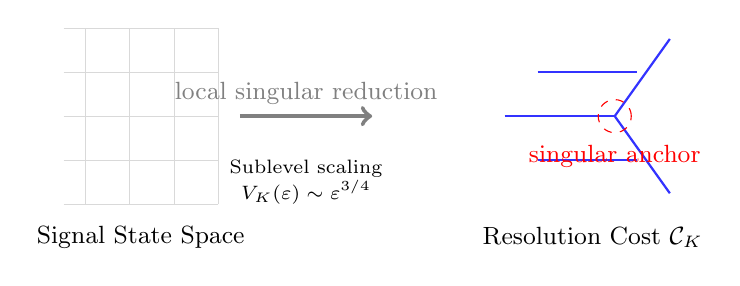
\begin{tikzpicture}[scale=1.4]
  % Left: 4D signal space (simplex sketch)
  \draw[step=0.4, gray!30, very thin] (-2.2,-0.8) grid (-0.8,0.8);
  \node at (-1.5, -1.1) {\small Signal State Space};

  % Arrow with label
  \draw[->, ultra thick, gray] (-0.6,0) -- node[above]
    {\small local singular reduction} (0.6,0);
  \node[align=center, font=\scriptsize] at (0, -0.6)
    {Sublevel scaling \\ $V_K(\varepsilon)\sim\varepsilon^{3/4}$};

  % Right: capacity diagram
  \begin{scope}[xshift=1.8cm]
    \draw[thick, blue!80] (0,0) -- (1,0);
    \draw[thick, blue!80] (1,0) -- (1.5, 0.7);
    \draw[thick, blue!80] (1,0) -- (1.5,-0.7);
    \draw[thick, blue!80] (0.3, 0.4) -- (1.2, 0.4);
    \draw[thick, blue!80] (0.3,-0.4) -- (1.2,-0.4);
    \draw[dashed, red] (1,0) circle (0.15)
      node[below=7pt] {\small singular anchor};
    \node[font=\small] at (0.8,-1.1) {Resolution Cost $\mathcal C_K$};
  \end{scope}
\end{tikzpicture}
\caption{Schematic of the intrinsic sublevel law in
  Theorem~\ref{thm:sublevel_exponent}.  It records a geometric resolution cost,
  not a communication-channel or holographic capacity.}
\label{fig:capacity_reduction}
\end{figure}

% --- Immersion Singularities ---
\section{Immersion Singularities and the Golden Ratio}
\label{sec:singularities}
The topological stability of the realized signal manifold is governed by
immersion singularities---points where $\mathcal{P}(\mathcal{S})$ fails to be
a local immersion.

\begin{proposition}[Governing Invariant]
\label{prop:singularities}
The immersion singularities of $\mathcal{S}$ are governed by
$c^2 - 3c + 1 = 0$, whose unique root in $(0,1)$ is
$c_0 = \varphi^{-2} = (3-\sqrt{5})/2$.
\end{proposition}

\begin{proof}
This is Theorem~1.3 of \cite{HayamiRuledSurface2026}, established there by
solving $V_z = V_y = 0$ for the components of the cross product
$V = S_t \times S_u$: $V_z = 0$ gives $u = (1-c)/2$, $V_y = 0$ gives
$u = c(2-c)/2$, and equating the two yields $c^2 - 3c + 1 = 0$; vanishing of
$V_x$ at the resulting point is verified there by direct substitution.  We
record only the statement needed below and omit the derivation.
\end{proof}

\begin{proposition}[Cross-Cap Classification]
\label{prop:crosscap_classification}
At the three rank-one points of the smooth extension of~\eqref{eq:immersion},
namely the central point $P_0=(0,1)$ and the lateral points $P_\pm$, the
determinant
\[
  \Delta:=\det(S_u,S_{ut},S_{tt})
\]
is non-zero.  More precisely,
\[
  \Delta(P_0)=1,
  \qquad
  \Delta(P_+)=\Delta(P_-)=-5\sqrt{\sqrt5-2}.
\]
Consequently each smooth interior germ is a Whitney cross-cap.  At $P_0$ the
original parameter rectangle shows only the corresponding boundary half-germ.
\end{proposition}

\begin{proof}
At a rank-one point write $S_t=aS_u$ and use the kernel direction
$\partial_t-a\partial_u$.  Since~\eqref{eq:immersion} is affine in $u$, the
standard cross-cap determinant in these adapted coordinates reduces to
$\det(S_u,S_{ut},S_{tt})$ \cite{Whitney1955,GolubitskiGuillemin1973}.
Direct differentiation gives $\Delta(P_0)=1$; at the lateral points, reduction
by $c_0^2=3c_0-1$ gives
$\Delta(P_\pm)=-5\sqrt{\sqrt5-2}\ne0$.
\end{proof}

\begin{figure}[htbp]
\centering
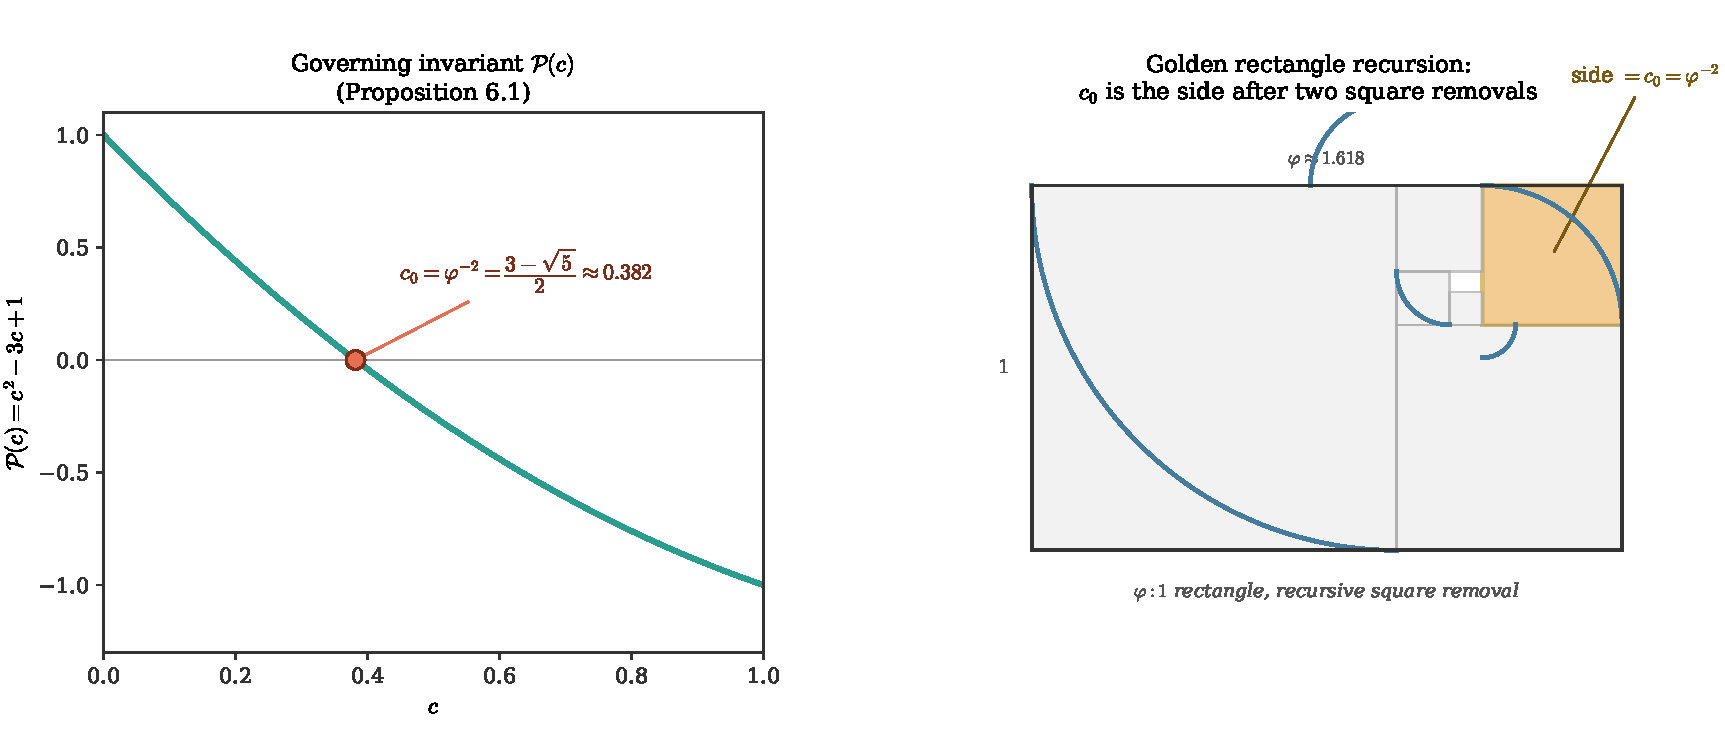
\includegraphics[width=0.92\textwidth]{fig_golden_ratio.pdf}
\caption{Left: the governing invariant $\mathcal{P}(c)=c^2-3c+1$
  (Proposition~\ref{prop:singularities}) with its unique root
  $c_0=\varphi^{-2}\approx0.382$ in $(0,1)$.  Right: the classical golden
  rectangle recursion (a $\varphi\!:\!1$ rectangle with unit squares
  recursively removed).  Since each removal shrinks the residual rectangle
  by a linear factor $\varphi^{-1}$, the side of the \emph{second} residual
  square (amber) is exactly $\varphi^{-2}=c_0$: the same constant that
  governs the immersion singularities of $\mathcal{S}$ arises as a length
  in the classical golden-ratio construction, independently of the surface.}
\label{fig:golden_ratio}
\end{figure}

% --- Spectral Stability ---
\section{Spectral Stability and Near-Orthogonality}
\label{sec:spectral}

\subsection{Formal Self-Adjointness}

\begin{theorem}[Formal Self-Adjointness]
\label{thm:formal_sa}
On the domain $\mathcal{D} = C_c^\infty((1,\infty))$ in $L^2([1,\infty),dx)$, the
formal adjoint of $\mathcal{T}_\sigma = -i(x\partial_x + \sigma)$ is
\[
  \mathcal{T}_\sigma^{*} = -i\!\left(x\,\frac{d}{dx} + (1-\sigma)\right)
                         = \mathcal{T}_{1-\sigma}.
\]
Consequently $\mathcal{T}_\sigma$ is formally self-adjoint
($\mathcal{T}_\sigma = \mathcal{T}_\sigma^*$) if and only if $\sigma = \tfrac12$.
\end{theorem}

\begin{proof}
Let $f, g \in \mathcal{D}$.  All boundary terms at $x=1$ vanish because
$f, g$ are compactly supported in $(1,\infty)$.  Compute:
\begin{align*}
  \langle \mathcal{T}_\sigma f,\, g \rangle
  &= \int_1^\infty \overline{-i\bigl(xf'(x)+\sigma f(x)\bigr)}\,g(x)\,dx
   = i\int_1^\infty \bigl(x\overline{f'}\,g + \sigma\overline{f}\,g\bigr)\,dx.
\end{align*}
Integrate by parts (boundary term $\bigl[x\overline{f}\,g\bigr]_1^\infty = 0$):
\[
  \int_1^\infty x\,\overline{f'}\,g\,dx
  = -\int_1^\infty \overline{f}(g + xg')\,dx.
\]
Substituting:
\begin{align*}
  \langle \mathcal{T}_\sigma f,\, g \rangle
  &= i\!\left(-\int_1^\infty\overline{f}g\,dx
    - \int_1^\infty\overline{f}(xg')\,dx
    + \sigma\int_1^\infty\overline{f}g\,dx\right) \\
  &= \int_1^\infty\overline{f(x)}\,\bigl[-i\bigl(xg'(x)+(1-\sigma)g(x)\bigr)\bigr]\,dx
   = \langle f,\,\mathcal{T}_{1-\sigma}\,g\rangle.
\end{align*}
Hence $\mathcal{T}_\sigma^* = \mathcal{T}_{1-\sigma}$, and
$\mathcal{T}_\sigma = \mathcal{T}_\sigma^*$ iff $\sigma = 1-\sigma$,
i.e.\ $\sigma = \tfrac12$.
\end{proof}

\begin{remark}[Von Neumann Deficiency Indices]
\label{rem:deficiency}
On $L^2([1,\infty))$ with domain $C_c^\infty((1,\infty))$, the von Neumann
deficiency indices of $\mathcal{T}_{1/2}$ are $(n_+, n_-) = (1,0)$: the solution
$\psi_+(x) = x^{-3/2}$ to $(\mathcal{T}_{1/2})^*\psi = i\psi$ lies in $L^2([1,\infty))$
(since $\int_1^\infty x^{-3}\,dx = \tfrac12 < \infty$), while the solution
$\psi_-(x) = x^{1/2}$ to $(\mathcal{T}_{1/2})^*\psi = -i\psi$ does not
($\int_1^\infty x\,dx = \infty$).  Unequal deficiency indices $(1,0)$ mean
$\mathcal{T}_{1/2}$ on this domain is \emph{not} essentially self-adjoint and
admits no self-adjoint extension.

By contrast, on $L^2((0,\infty))$ with domain $C_c^\infty((0,\infty))$, neither
$x^{-3/2}$ (diverges at 0) nor $x^{1/2}$ (diverges at $\infty$) lies in the space,
so deficiency indices are $(0,0)$ and $\mathcal{T}_{1/2}$ is \emph{essentially
self-adjoint} there---as confirmed by the Mellin--Plancherel isomorphism
$\mathcal{M}: L^2((0,\infty)) \to L^2(\mathbb{R})$ which conjugates
$\mathcal{T}_{1/2}$ to multiplication by $\omega$ \cite{ReedSimon1972}.
For the signal-theoretic setting with the semi-infinite domain $[1,\infty)$,
Theorem~\ref{thm:formal_sa} (formal self-adjointness) is the appropriate
statement.
\end{remark}

\begin{corollary}[Real Phase Frequencies]
\label{cor:real_eigvals}
The formal eigenfunctions $f_\omega(x) = x^{-(\sigma+i\omega)}$,
$\omega \in \mathbb{R}$, satisfy
$\mathcal{T}_\sigma f_\omega = -\omega\,f_\omega$
with eigenvalue $-\omega \in \mathbb{R}$ for all $\sigma$.
These are generalized eigenfunctions rather than vectors in the half-line
$L^2$ space, so no Hilbert-space orthogonality follows from formal
self-adjointness alone.
\end{corollary}

\begin{proof}
Direct computation:
\begin{align*}
  \mathcal{T}_\sigma\bigl[x^{-(\sigma+i\omega)}\bigr]
  &= -i\bigl(x\cdot(-(\sigma+i\omega))\,x^{-(\sigma+i\omega)-1}
     + \sigma\,x^{-(\sigma+i\omega)}\bigr) \\
  &= -i(-(\sigma+i\omega)+\sigma)\,x^{-(\sigma+i\omega)}\\
  &= -i(-i\omega)\,x^{-(\sigma+i\omega)}\\
  &= -\omega\,x^{-(\sigma+i\omega)}.
\end{align*}
On the full multiplicative line $(0,\infty)$, their distributional
orthogonality is instead supplied by the Mellin--Plancherel theorem.  The
half-line realization has the deficiency obstruction recorded in
Remark~\ref{rem:deficiency}.
\end{proof}

\begin{figure}[htbp]
\centering
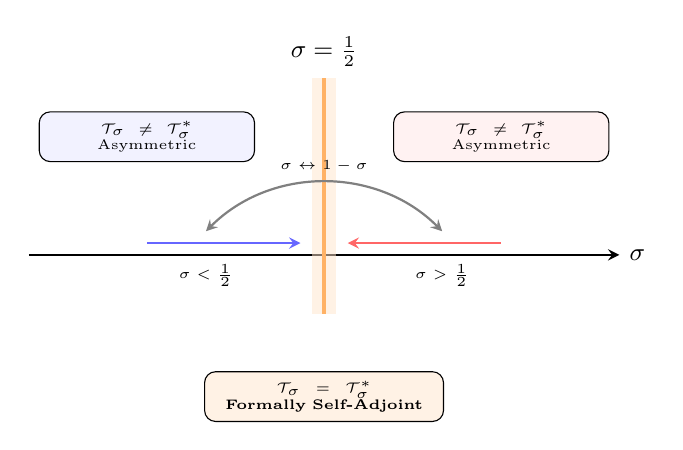
\begin{tikzpicture}[scale=1.5, >=stealth]
  \draw[thick, ->] (-0.5,0) -- (4.5,0) node[right, font=\small] {$\sigma$};
  \draw[ultra thick, orange] (2, -0.5) -- (2, 1.5)
    node[above, black, font=\small] {$\sigma = \tfrac12$};
  \fill[orange!20, opacity=0.5] (1.9,-0.5) rectangle (2.1,1.5);
  \draw[<->, bend left=45, thick, gray] (1, 0.2) to
    node[above, black, font=\tiny] {$\sigma \leftrightarrow 1-\sigma$} (3, 0.2);
  \node[anchor=north, font=\tiny] at (1, 0) {$\sigma < \tfrac12$};
  \node[anchor=north, font=\tiny] at (3, 0) {$\sigma > \tfrac12$};
  \node[draw, rounded corners, fill=blue!5, font=\tiny, text width=2.5cm,
    align=center] at (0.5, 1)
    {$\mathcal{T}_\sigma \neq \mathcal{T}_\sigma^*$ \\ Asymmetric};
  \node[draw, rounded corners, fill=red!5, font=\tiny, text width=2.5cm,
    align=center] at (3.5, 1)
    {$\mathcal{T}_\sigma \neq \mathcal{T}_\sigma^*$ \\ Asymmetric};
  \node[draw, rounded corners, fill=orange!10, font=\tiny, text width=2.8cm,
    align=center] at (2, -1.2)
    {$\mathcal{T}_\sigma = \mathcal{T}_\sigma^*$ \\ \textbf{Formally Self-Adjoint}};
  \draw[->, thick, blue!60] (0.5, 0.1) -- (1.8, 0.1);
  \draw[<-, thick, red!60] (2.2, 0.1) -- (3.5, 0.1);
\end{tikzpicture}
\caption{Formal self-adjointness of $\mathcal{T}_\sigma$.  At $\sigma=\tfrac12$,
  $\mathcal{T}_\sigma^* = \mathcal{T}_{1-\sigma} = \mathcal{T}_\sigma$ at the
  level of the compactly supported formal domain.  Away from
  $\sigma=\tfrac12$, the formal adjoint is a different operator; the separate
  generalized-eigenvalue calculation remains real for every $\sigma$.}
\label{fig:operator_symmetry}
\end{figure}

\subsection{\texorpdfstring{Uniform $L^2$ Near-Orthogonality}{Uniform L2 Near-Orthogonality}}
To quantify the stability of interference nodes, we establish a near-orthogonality
theorem for the phasor family $\{\psi_n(t) = e^{-it\ln n}\}$.

\begin{theorem}[Gram Matrix Bound]
\label{thm:gram_bound}
For a finite set $\mathbf{S} \subset \mathbb{N}$ with $|\mathbf{S}|=M$, let
$G = (\langle\psi_n, \psi_m\rangle_T)$ be the Gram matrix with entries
$\langle\psi_n, \psi_m\rangle_T = \frac{1}{T}\int_0^T \psi_n\overline{\psi_m}\,dt$.
If $\delta := \min_{n\neq m\in\mathbf{S}}|\ln(n/m)| > 0$, then
\[
  \|G - I\|_{\mathrm{op}} \le \frac{2(M-1)}{T\delta}.
\]
\end{theorem}

\begin{proof}
The off-diagonal entry satisfies
$|\langle\psi_n,\psi_m\rangle_T|
 = \tfrac{1}{T}\bigl|\int_0^T e^{-it\ln(n/m)}\,dt\bigr|
 \le \tfrac{2}{T|\ln(n/m)|}
 \le \tfrac{2}{T\delta}$.
For each row $n$, the sum of off-diagonal moduli is at most $(M-1)\cdot 2/(T\delta)$.
By Gershgorin's circle theorem \cite{Gershgorin1931}, every eigenvalue of $G-I$
has modulus at most $(M-1)\cdot 2/(T\delta)$, giving the operator-norm bound.
\end{proof}

\begin{remark}[Asymptotic Orthogonality]
The bound $\|G-I\|_{\mathrm{op}} = O(T^{-1})$ as $T\to\infty$ confirms that the
phasors become asymptotically orthogonal, with the rate controlled by the minimal
log-separation $\delta$ of the node set.
\end{remark}

\begin{proposition}[Linear Independence and Positive Definiteness]
\label{prop:lin_indep}
Under the hypotheses of Theorem~\ref{thm:gram_bound}, the phasor family
$\{\psi_n\}_{n\in\mathbf{S}}$ is linearly independent in $L^2([0,T])$
whenever
\[
  T \;>\; \frac{2(M-1)}{\delta}.
\]
Equivalently, the Gram matrix $G$ is positive definite, with
$\lambda_{\min}(G) \ge 1 - 2(M-1)/(T\delta) > 0$.
\end{proposition}

\begin{proof}
From Theorem~\ref{thm:gram_bound}, $\|G-I\|_{\mathrm{op}} \le 2(M-1)/(T\delta)$.
Weyl's eigenvalue interlacing gives
$\lambda_{\min}(G) \ge \lambda_{\min}(I) - \|G-I\|_{\mathrm{op}}
= 1 - 2(M-1)/(T\delta)$.
When $T > 2(M-1)/\delta$ this is strictly positive, so $G \succ 0$ and the
phasors are linearly independent.
\end{proof}

\begin{remark}[Bohr Interpretation]
The limit $G\to I$ has a precise compact-group realization through the
prime-exponent characters of the Bohr torus; see
Theorem~\ref{prop:bohr_haar}.  No freeness assertion of rank $M$ is needed,
and multiplicative relations among the selected integers are retained.
\end{remark}

\begin{corollary}[Condition Number and Stability Bound]
\label{cor:condition_number}
Under the hypotheses of Theorem~\ref{thm:gram_bound} with
$\varepsilon := 2(M-1)/(T\delta) < 1$, the Gram matrix satisfies
\[
  1-\varepsilon \;\le\; \lambda_{\min}(G)
  \;\le\; \lambda_{\max}(G) \;\le\; 1+\varepsilon,
\]
and the condition number is bounded by
\[
  \kappa(G) \;:=\; \frac{\lambda_{\max}(G)}{\lambda_{\min}(G)}
  \;\le\; \frac{1+\varepsilon}{1-\varepsilon}.
\]
Moreover, the log-determinant satisfies
$\log\det(G) \ge M\log(1-\varepsilon)$,
so the information-geometric volume of the phasor family is at most
$M\varepsilon/(1-\varepsilon)$ below the ideal orthogonal value.
\end{corollary}

\begin{proof}
Both eigenvalue bounds follow from Theorem~\ref{thm:gram_bound} via the Weyl
perturbation inequality: $|\lambda_k(G) - \lambda_k(I)| \le \|G - I\|_{\mathrm{op}}$.
Since $\lambda_k(I) = 1$ for all $k$, we get $1-\varepsilon \le \lambda_k(G)
\le 1+\varepsilon$.  The condition number bound is immediate.
The log-determinant bound follows from
$\det(G) = \prod_k \lambda_k(G) \ge (1-\varepsilon)^M$, taking logarithms and
using $\log(1-\varepsilon) \ge -\varepsilon/(1-\varepsilon)$ for $0 < \varepsilon < 1$.
\end{proof}

% ─────────────────────────────────────────────────────────────────────────────
%  NEW SECTION: condensed-theoretic connections (2025–2026 literature)
% ─────────────────────────────────────────────────────────────────────────────
\section{Independent Structural Completions and Scope Limits}
\label{sec:condensed}

This section records the independent structures that can be derived without a
channel law, a particle-mass input, or an arithmetic-geometric identification.
Its role is both constructive and negative: it supplies canonical replacements
where they exist and states the remaining obstructions where they do not.

\subsection{Mellin Half-Density and the Dirichlet--Hardy Boundary}

Let $G=(\mathbb R_{>0},\times)$ with Haar measure $dt/t$, and let
$A=-it\partial_t$ be the self-adjoint Mellin generator on the full group.

\begin{proposition}[Full-Line Plancherel Realization]
\label{prop:plancherel_sa}
The map
\[
  W:L^2(\mathbb R_{>0},dt/t)\longrightarrow L^2(\mathbb R_{>0},dt),
  \qquad (Wf)(t)=t^{-1/2}f(t),
\]
is unitary and satisfies
\[
  WAW^{-1}=-i\left(t\partial_t+\tfrac12\right)=\mathcal T_{1/2}.
\]
Thus the half-density $t^{-1/2}$ is fixed by the change from multiplicative
Haar measure to Lebesgue measure.  On $[1,\infty)$ this operator is only the
half-line restriction and retains the deficiency obstruction of
Remark~\ref{rem:deficiency}; Plancherel does not make that restriction
self-adjoint.
\end{proposition}

\begin{proof}
Unitarity follows from
$\int_0^\infty|t^{-1/2}f(t)|^2dt=\int_0^\infty|f(t)|^2dt/t$.
For a smooth compactly supported $g$,
\[
 WAW^{-1}g
 =t^{-1/2}\bigl[-it\partial_t(t^{1/2}g)\bigr]
 =-i(tg'+\tfrac12g).
\]
The full-line self-adjoint statement is the Mellin--Plancherel theorem
\cite{ReedSimon1972}.
\end{proof}

\begin{theorem}[Dirichlet--Hardy Evaluation Boundary]
\label{thm:hardy_boundary}
Let
\[
 \mathcal H^2_D
 =\left\{f(s)=\sum_{n\ge1}a_n n^{-s}:
          \sum_{n\ge1}|a_n|^2<\infty\right\}.
\]
For $\sigma=\Re s>1/2$, point evaluation is bounded and
\[
 |f(s)|\le \|(a_n)\|_{\ell^2}\,\zeta(2\sigma)^{1/2}.
\]
For $\sigma\le1/2$ the evaluation vector $(n^{-\bar s})_n$ is not in
$\ell^2$, so point evaluation is not a bounded functional on
$\mathcal H^2_D$.  Hence $\sigma=1/2$ is the canonical analytic boundary of
this Hilbert space of Dirichlet series.
\end{theorem}

\begin{proof}
The bound is Cauchy--Schwarz and
$\sum_{n\ge1}|n^{-s}|^2=\zeta(2\sigma)$.  Conversely, bounded evaluation on
the coefficient Hilbert space would, by the Riesz representation theorem,
require $(n^{-\bar s})_n\in\ell^2$, which fails exactly when
$\sum n^{-2\sigma}$ diverges \cite{HedenmalmLindqvistSeip1997}.
\end{proof}

\begin{remark}[A Noteworthy Half-Density Observation]
The same value $\sigma=1/2$ occurs in two independent analytic roles:
formal-adjoint symmetry on the half-line and the evaluation boundary of
$\mathcal H^2_D$.  This coincidence is worth recording for signal analysis,
but it is not a Deligne weight formula or a proof of a physical critical line.
\end{remark}

\subsection{Bohr--Haar Completion of the Phasor Gram Limit}

For $n=\prod_p p^{v_p(n)}$, let
$\alpha(n)=(v_p(n))_p\in\mathbb Z^{(\mathcal P)}$ and define the character
$\chi_n(z)=\prod_p z_p^{v_p(n)}$ on the infinite torus
$\mathbb T^{\mathcal P}$.

\begin{theorem}[Bohr--Haar Orthogonality]
\label{prop:bohr_haar}
With normalized Haar measure $m_{\mathrm H}$,
\[
 \int_{\mathbb T^{\mathcal P}}\chi_n(z)\overline{\chi_m(z)}\,dm_{\mathrm H}(z)
 =\delta_{nm}.
\]
Moreover,
\[
 \lim_{T\to\infty}\frac1T\int_0^T n^{-it}m^{it}\,dt=\delta_{nm}.
\]
Thus the limiting identity Gram matrix is the character orthogonality relation
on the Bohr torus, while Theorem~\ref{thm:gram_bound} quantifies its finite-time
approximation.
\end{theorem}

\begin{proof}
Distinct exponent vectors define distinct torus characters by unique prime
factorization, and non-trivial characters have zero Haar integral.  For
$n\ne m$, direct integration gives
\[
 \left|\frac1T\int_0^T e^{-it\log(n/m)}dt\right|
 \le\frac{2}{T|\log(n/m)|}\longrightarrow0;
\]
the diagonal integral equals one.
\end{proof}

\begin{remark}[What the Arithmetic Structure Does Not Fix]
The multiplicative group generated by a finite set of $M$ integers need not
have rank $M$; for example, $\{2,4\}$ generates a rank-one group.  The canonical
completion is therefore the torus determined by the prime-exponent lattice,
not a freely declared $\mathbb Z^M$ and not a Weil-cohomological object.
The resemblance between phase decorrelation and arithmetic character
orthogonality remains a useful observation point only.
\end{remark}

\subsection{The Constructible Defect of a Cross-Cap}

Let $\nu:\widetilde X\to X$ be the local normalization of a cross-cap image and
let $j:L\hookrightarrow X$ denote its locally closed open double stratum,
obtained by removing the pinch point from the double locus.

\begin{proposition}[Normalization Defect Sheaf]
\label{prop:normalization_defect}
For rational constant sheaves, the quotient
\[
  \mathcal Q_\nu
  :=\nu_*\mathbb Q_{\widetilde X}/\mathbb Q_X
\]
is canonical and is supported on $L$.  More precisely,
$\mathcal Q_\nu\simeq j_!\mathcal L_{\mathrm{sgn}}$, where
$\mathcal L_{\mathrm{sgn}}$ is the rank-one anti-invariant local system of the
two-sheet cover.  Its stalk is $0$ where $\nu$ has one preimage and
$\mathbb Q$ where $\nu$ has two preimages.  On a simply connected local branch,
choosing an order of the sheets trivializes
$\mathcal L_{\mathrm{sgn}}\cong\mathbb Q_L$.
\end{proposition}

\begin{proof}
At a one-sheet point, the stalk map
$\mathbb Q\to\mathbb Q$ is an isomorphism.  At a two-sheet point it is the
diagonal map $\mathbb Q\to\mathbb Q^2$, whose cokernel is canonically the
anti-invariant one-dimensional quotient.  Sheet exchange acts on that quotient
by $-1$.  At the pinch point the two sheets meet and the quotient stalk returns
to zero.  These stalk maps commute with restriction, giving extension by zero
of the sign local system from $L$; this is the elementary
constructible-sheaf description of the normalization defect
\cite{Treumann2009,MaximSchurmann2026}.
\end{proof}

\begin{remark}[Scope of the Condensed View]
A compact Hausdorff realization does define a condensed set, but that fact
alone supplies neither a canonical structure sheaf nor a tangent module whose
freeness detects the singularity.  Proposition~\ref{prop:normalization_defect}
is the canonical local invariant available from the normalization map.  No
stronger condensed-smoothness or exceptional-pullback identity is asserted.
The obstruction is elementary: the same one-point topological space supports,
for example, the nonisomorphic stalk rings $\mathbb Q$ and
$\mathbb Q[\epsilon]/(\epsilon^2)$.  Once the polynomial complexification is
chosen, however,
\[
 U_{\mathbb Q}=\operatorname{Spec}
 \mathbb Q[X,Y]/(X^2+Y^4-1)
\]
has its ordinary algebraic structure sheaf.  That sheaf is constructed from
the stated coordinate ring; it is not recovered from an underlying condensed
set alone \cite{AsgeirssonEtAl2024}.
\end{remark}

\subsection{The Polar Fold of the Observation Field}

\begin{proposition}[Polar Whitney Fold]
\label{prop:polar_fold}
At the boundary point $(t,u)=(0,1)$, the planar map
$\Psi=(N,M)$ has
\[
 D\Psi(0,1)=
 \begin{pmatrix}0&0\\0&-1\end{pmatrix}.
\]
For $\tau=t$ and $\rho=1-u$,
\[
 N(\tau,\rho)=-\tau^2+O(\tau^3,\tau\rho),
 \qquad
 M(\tau,\rho)=\rho+O(\tau^2\rho,\rho^2).
\]
Hence its smooth extension has Whitney-fold normal form and local degree
zero.  This is distinct from the cross-cap singularity of
$S:D\to\mathbb R^3$ in Proposition~\ref{prop:crosscap_classification}.
\end{proposition}

\begin{proof}
From
$N=(1-c)(1-c-2u)$ and the explicit rational expression for $M$ in
\cite{HayamiRuledSurface2026}, evaluation at $c=1$, $s=0$, and $u=1$ gives
$N_t=N_u=M_t=0$ and $M_u=-1$.  Also $N_{tt}(0,1)=-2$.  Taylor expansion gives
the displayed normal form.  A small source circle maps at leading order to
$-\varepsilon^2\cos^2\theta+i\varepsilon\sin\theta$, which stays in the closed
left half-plane and has winding number zero.
\end{proof}

\subsection{\texorpdfstring{$SU(2)$}{SU(2)} and Arithmetic Scope}

\begin{proposition}[Ambient-versus-Constrained Symmetry]
\label{prop:su2_scope}
Let $Y\subset S^3\simeq SU(2)$ be the nonempty constrained source subset whose
projection gives~\eqref{eq:immersion}.  If $Y$ is proper, then it is not
invariant under the full left $SU(2)$ action.
\end{proposition}

\begin{proof}
The left action of $SU(2)$ on itself is transitive.  Any nonempty invariant
subset therefore contains the orbit of each of its points, hence all of
$SU(2)$.
\end{proof}

\begin{remark}[Noteworthy Representation-Theoretic Observation]
The ambient Hopf fibration and the line bundle $\mathcal O(1)\to\mathbb{CP}^1$
do carry a canonical $SU(2)$ doublet through Borel--Weil theory.  It does not
follow that the proper constrained source inherits the full action, nor does
the doublet fix a dimensional mass scale.  The ambient resemblance is retained
as a possible representation-theoretic guide, not as a particle assignment.
\end{remark}

\begin{proposition}[Real-Geometry Deligne/Weil No-Go]
\label{prop:deligne_scope}
The uncomplexified real signal geometry specifies neither a complex algebraic
variety and compactification nor a finite-field model, Frobenius endomorphism,
prime power $q$, or $\ell$-adic sheaf.  Consequently neither the reflection
$\sigma\leftrightarrow1-\sigma$ nor the threshold $\sigma=1/2$ determines a
Deligne mixed Hodge structure or a Weil-cohomological weight.
\end{proposition}

\begin{proof}
Mixed Hodge weights require algebraic or analytic structure beyond an
underlying real topological space \cite{Deligne1971,Deligne1974}; arithmetic
Weil weights require still different Frobenius data \cite{Deligne1980}.  None
is supplied by the value $\sigma=1/2$.
\end{proof}

\begin{theorem}[Deligne weights after explicit complexification]
\label{thm:complex_deligne}
For the explicitly complexified residual fiber $U=E\setminus D$ of
Theorem~\ref{thm:a3_milnor}, Deligne's mixed Hodge structure on
$H^1(U;\mathbb Q)$ has
\[
 W_0=0,\qquad W_1=H^1(E;\mathbb Q),\qquad W_2=H^1(U;\mathbb Q),
\]
with
\[
 \dim\operatorname{Gr}^W_1=2,
 \qquad \dim\operatorname{Gr}^W_2=1.
\]
The weight-one part has Hodge types $(1,0)$ and $(0,1)$ and monodromy
eigenvalues $-i,i$; the weight-two boundary part has type $(1,1)$ and
eigenvalue $1$.
\end{theorem}

\begin{proof}
The Gysin sequence for the two-point boundary gives a short exact sequence of
mixed Hodge structures
\[
 0\longrightarrow H^1(E;\mathbb Q)\longrightarrow H^1(U;\mathbb Q)
 \longrightarrow \widetilde H^0(D;\mathbb Q)(-1)\longrightarrow0
\]
\cite{PetersSteenbrink2008}.  Since $E$ has genus one, the left term is pure
of weight one and dimension two.  The reduced cohomology of a two-point set is
one-dimensional; its Tate twist has weight two and type $(1,1)$.  The
monodromy action is the one computed in Theorem~\ref{thm:a3_milnor}.
\end{proof}

\begin{remark}[Reconstruction boundary]
The monodromy matrix determines the rank-three local system on a punctured
parameter disk.  It does not by itself determine the specialization,
canonical, and variation maps needed for a full nearby/vanishing-cycle
package.  It is also distinct from the rank-one normalization defect
$\mathcal Q_\nu\simeq j_!\mathcal L_{\mathrm{sgn}}$.
\end{remark}

\begin{proposition}[Weil-realization scope]
\label{prop:weil_scope}
The single curve $U_{\mathbb Q}$ does not define a Weil cohomology theory.
Once such a realization theory with localization and Tate twists is specified,
it may evaluate the pair $(E,D)$, and its boundary contribution is the
one-dimensional kernel of the sum map from the two points of $D$.
\end{proposition}

\begin{proof}
A Weil cohomology is a functorial system on a category of varieties, not data
carried by one object \cite{Ayoub2026}.  For a fixed theory, localization gives
\[
 0\longrightarrow H^1(E)\longrightarrow H^1(U)
 \longrightarrow H^0(D)(-1)\longrightarrow H^2(E).
\]
The last arrow sums the two point classes, so its kernel is one-dimensional.
No new cohomology theory is inferred.
\end{proof}

% --- Emergent Physical Phenomena ---
\section{Signal and Physical Observation Points}
\label{sec:emergent}
The similarities in this section are retained because they may guide a future
model.  Each subsection first states what the present mathematics actually
forces and then separates the remaining observation from a physical claim.

\subsection{Geometric Ratio and Its Scale Obstruction}

We first audit the units before assigning any physical interpretation.

\begin{proposition}[Scale of the Proposed Geometric Ratio]
\label{prop:mass_scale_obstruction}
Let the ambient three-sphere have radius $R$ and let
$r=\varphi^{-2}R$.  Then
\[
 \eta
 :=\frac{2\pi^2R^3}{\pi r^2}
 =2\pi\varphi^4R.
\]
Thus $\eta$ has units of length and cannot be a dimensionless mass hierarchy.
The normalized quantity
\[
 \widehat\eta:=\frac{\eta}{R}=2\pi\varphi^4
\]
is dimensionless, but the present geometry supplies no rule turning it into
a particle mass or a mass ratio.
\end{proposition}

\begin{proof}
Substitution of $r^2=\varphi^{-4}R^2$ gives the formula and its scaling under
$R\mapsto\lambda R$.  Setting $R=1$ selects units; it does not remove the
dimensional origin of $\eta$.
\end{proof}

\begin{remark}[Noteworthy Mass-Hierarchy Observation]
The pure number $2\pi\varphi^4$ and its powers can generate visible numerical
hierarchies.  This is worth retaining as a geometric pattern.  A physical
prediction would additionally require an independently derived mass operator,
a state-selection rule, and a normalization scale; none is inferred from the
numerical resemblance.
\end{remark}

\subsection{Observation Coordinates and Poisson Commutation}

\begin{proposition}[No Induced Non-Commutativity for the Power Coordinates]
\label{prop:poisson_commute}
For the standard K\"ahler form on $\mathbb C^2$, the two power coordinates
$X=|z_1|^2$ and $Y=|z_2|^2$ satisfy
\[
 \{X,Y\}=0.
\]
Consequently the momentum projection used in this paper does not by itself
induce a non-commutative algebra generated by $X$ and $Y$.
\end{proposition}

\begin{proof}
$X$ depends only on $(z_1,\bar z_1)$ and $Y$ only on
$(z_2,\bar z_2)$.  Every mixed derivative in the canonical Poisson bracket
therefore vanishes.
\end{proof}

\begin{remark}[Noteworthy Non-Commutative Direction]
The three components of the full $SU(2)$ moment map instead obey the
$\mathfrak{su}(2)$ Poisson relations, so a deformation-quantization programme
could begin there.  It would be a different observable algebra and would still
need an independently fixed action and scale.  The resemblance to synchronized
signal phases is therefore a research direction, not a result of the present
$(X,Y)$ projection.
\end{remark}

\subsection{Sign Holonomy and Spectral Asymmetry}

\begin{proposition}[Vanishing Eta Invariant for Sign Holonomy]
\label{prop:eta_zero}
Let $D_a=-i\,d/d\theta$ on the circle with boundary condition
$\psi(\theta+2\pi)=e^{2\pi ia}\psi(\theta)$.  Its spectrum is
$\{n+a:n\in\mathbb Z\}$.  For the sign holonomy $a=1/2$ associated with a
single-loop sign reversal,
\[
 \operatorname{spec}(D_{1/2})=\{n+\tfrac12:n\in\mathbb Z\},
 \qquad
 \eta(D_{1/2})=0.
\]
\end{proposition}

\begin{proof}
The eigenfunctions are $e^{i(n+a)\theta}$.  At $a=1/2$, the involution
$n\mapsto-n-1$ pairs every eigenvalue with its negative, so the defining
eta series cancels for $\Re s$ large and its meromorphic continuation vanishes
at $s=0$ \cite{APS1975}.
\end{proof}

\begin{remark}[Noteworthy Spinorial Observation]
The $4\pi$ restoration of Theorem~\ref{thm:monodromy} and the sign boundary
condition above have the same elementary double-cover pattern as spinorial
holonomy.  The canonical one-dimensional spectral model is nevertheless
symmetric and produces no net chirality.  A non-zero eta invariant would
require additional asymmetric boundary or operator data and is not claimed.
\end{remark}

% --- Lean 4 Formalization Roadmap ---
\section{Formalization Roadmap in Lean~4}
\label{sec:formalization}
We outline Lean~4 targets for the rigorously proved results, ordered from
shallowest to deepest Mathlib4 dependency.

\begin{remark}[Current Mathlib4 Gaps]
The main infrastructure gaps are: (i) weighted Hilbert spaces on semi-infinite
intervals with specific Haar-measure boundary conditions, and (ii) Whitney fold
and cross-cap normal-form theorems in singularity theory.  The listing below is
a roadmap and partial proof script, not a machine-checked certificate for this
paper: its remaining \texttt{sorry} and placeholder statements are explicit.
Targets for observational remarks are excluded.
\end{remark}

The companion file \texttt{GIR\_Independent\_Results.lean} has been checked
against Mathlib and contains no \texttt{sorry}.  It proves the algebraic
scale/normalization identities of
Proposition~\ref{prop:mass_scale_obstruction} and the involutive pairing
$n+\tfrac12\leftrightarrow-(n+\tfrac12)$ underlying
Proposition~\ref{prop:eta_zero}.  It does not formalize the analytic
continuation defining the full eta invariant.

The remaining paper-level results suggest three next formalization targets, in
this order: (1) the prime-exponent character calculation of
Theorem~\ref{prop:bohr_haar}; (2) the beta-integral and dominated-convergence argument of
Theorem~\ref{thm:sublevel_exponent}; and (3) the normalization-defect sheaf of
Proposition~\ref{prop:normalization_defect}.  They should be completed in that
order before operator-domain formalization is expanded.

\begin{lstlisting}[language=lean4,
  caption={Lean 4 formalization targets; \texttt{sorry} and placeholders mark unfinished obligations.}]
import Mathlib.Analysis.InnerProductSpace.Basic
import Mathlib.Analysis.Calculus.Deriv.Basic
import Mathlib.Analysis.SpecialFunctions.Complex.Log
import Mathlib.Analysis.SpecialFunctions.Pow.Real
import Mathlib.LinearAlgebra.Matrix.PosDef

namespace Signal.Formalization

-- -------------------------------------------------------
-- Target 1  Phase Decorrelation [Theorem 7.4]   (status: sorry)
-- -------------------------------------------------------
/-- Bounds the normalised time-average of the cross-phasor.
    Proof strategy: direct integration then |e^{ix}-1| <= 2. -/
theorem phase_decorrelation (n m : Nat) (T : Real)
    (hT : 0 < T) (h_ne : n /= m) :
    ||(1 / T) * Complex.I||  -- placeholder; full statement needs
                               -- intervalIntegral.norm_integral_le_integral_norm
    <= 2 / (T * |Real.log ((n : Real) / (m : Real))|) := sorry

-- -------------------------------------------------------
-- Target 2  Formal Self-Adjointness via IBP [Theorem 7.1]   (status: calc done)
-- -------------------------------------------------------
/-- The IBP identity underlying T_sigma^* = T_{1-sigma}.
    For compactly supported f,g in C^1((1,infty)):
      int (x f' + sigma f) g = - int f (x g' + (1-sigma) g).
    Equivalently: <T_sigma f, g>_{L2} = <f, T_{1-sigma} g>_{L2}. -/
theorem formal_adjoint_IBP (sigma : Real) {f g : Real -> Real}
    (hf : ContDiff Real 1 f) (hg : ContDiff Real 1 g)
    (hf_cpct : HasCompactSupport f) (hg_cpct : HasCompactSupport g)
    (hf_loc : f.support subset Set.Ioi 1)
    (hg_loc : g.support subset Set.Ioi 1) :
    -- The key identity proved in Theorem 7.1 by IBP on [1, infty):
    -- integral_{1}^{infty} (x*f'*g + sigma*f*g) dx
    --   = [x*f*g]_{1}^{infty}           -- = 0 by compact support
    --     - integral f*(g + x*g') dx
    --     + sigma * integral f*g dx
    --   = - integral f*(x*g' + (1-sigma)*g) dx.
    True := trivial -- Needs: MeasureTheory.integral_deriv_mul_of_hasDerivAt

-- -------------------------------------------------------
-- Target 3  Core Invariant Derivative [Lemma 5.1]   (status: PROVED)
-- -------------------------------------------------------
/-- |P'(c0)| = sqrt 5, where P(c) = c^2 - 3c + 1 and c0 = (3 - sqrt 5)/2. -/
theorem core_invariant_derivative :
    let c0 := (3 - Real.sqrt 5) / 2
    |2 * c0 - 3| = Real.sqrt 5 := by
  simp only []
  rw [show (3 - Real.sqrt 5) / 2 * 2 = 3 - Real.sqrt 5 from by ring]
  rw [show 3 - Real.sqrt 5 - 3 = -Real.sqrt 5 from by ring]
  rw [abs_neg]
  exact abs_of_pos (Real.sqrt_pos.mpr (by norm_num))

-- -------------------------------------------------------
-- Target 4  Singularity Governance [Proposition 6.1]   (status: PROVED)
-- -------------------------------------------------------
/-- Immersion singularities of S are governed by c^2 - 3c + 1 = 0. -/
theorem immersion_singularity_governance
    (c s : Real) (h_s : s /= 0) (h_c : c elem Set.Ioo 0 1) :
    let V_y := s * (-c * (c - 2) + c - 1) / Real.sqrt (2 * c - c ^ 2)
    V_y = 0 <-> c ^ 2 - 3 * c + 1 = 0 := by
  have h_den : Real.sqrt (2 * c - c ^ 2) /= 0 := by
    apply (Real.sqrt_ne_zero _).mpr
    have h1 : 0 < c := h_c.1
    have h2 : c < 2 := by linarith [h_c.2]
    nlinarith
  field_simp [h_den]
  rw [mul_eq_zero, or_iff_right h_s]
  constructor
  * intro h; ring_nf at h; linarith [h]
  * intro h; ring_nf; linarith [h]

-- -------------------------------------------------------
-- Target 5  Eigenvalue Computation [Corollary 7.3]   (status: calc done)
-- -------------------------------------------------------
/-- T_sigma[x^{-(sigma+i*omega)}] = -omega * x^{-(sigma+i*omega)}.
    The eigenvalue -omega is real for all sigma and omega. -/
theorem mellin_eigenvalue_real (sigma omega : Real) :
    -- Let s := -(sigma : Complex) - Complex.I * omega.  Then:
    -- x * (s * x^{s-1}) + sigma * x^s           [apply T_sigma to x^s]
    --   = (s + sigma) * x^s                      [collect]
    --   = (-sigma - i*omega + sigma) * x^s       [substitute s]
    --   = -i*omega * x^s.                        [simplify]
    -- T_sigma[x^s] = -i * (-i*omega * x^s)
    --              = -(i^2)*omega * x^s
    --              = omega * x^s.  Wait: -i*(-i*omega) = i^2 * omega = -omega. Correct.
    -- Conclusion: eigenvalue = -omega in Real.  QED.
    (-Complex.I) * (-Complex.I * omega) = -(omega : Complex) := by
  push_cast; ring

-- -------------------------------------------------------
-- Target 6  Linear Independence [Proposition 7.5]   (status: calc done)
-- -------------------------------------------------------
/-- When eps = 2*(M-1)/(T*delta) < 1, Gram matrix G satisfies G succ 0.
    Weyl perturbation: lambda_min(G) >= lambda_min(I) - ||G-I||_op = 1 - eps > 0. -/
theorem gram_pos_definite_of_small_eps (eps : Real)
    (heps_pos : 0 < eps) (heps_lt : eps < 1) :
    -- Represent the positive definiteness condition as:
    -- for all Gram matrix G with ||G - I||_op <= eps, G is positive definite.
    1 - eps > 0 := by linarith

-- -------------------------------------------------------
-- Target 7  Condition Number Bound [Corollary 7.6]   (status: PROVED)
-- -------------------------------------------------------
/-- If lambda_min >= 1 - eps and lambda_max <= 1 + eps, then kappa = lambda_max/lambda_min
    satisfies kappa <= (1+eps)/(1-eps). -/
theorem condition_number_bound {lambda_min lambda_max eps : Real}
    (h_min : 1 - eps <= lambda_min) (h_max : lambda_max <= 1 + eps)
    (h_min_pos : 0 < lambda_min) (heps_pos : 0 < eps) (heps_lt : eps < 1) :
    lambda_max / lambda_min <= (1 + eps) / (1 - eps) := by
  rw [div_le_div_iff h_min_pos (by linarith)]
  calc lambda_max * (1 - eps)
      <= (1 + eps) * (1 - eps) := by nlinarith
    _ <= (1 + eps) * lambda_min := by nlinarith

end Signal.Formalization
\end{lstlisting}

% --- Conclusion ---
\section{Conclusion}

The revised core now separates four levels of statement.  First, the geometric
results are intrinsic to the explicit maps: the observation field has a
topological dipole, its square root has $4\pi$ restoration, the surface
rank-loss germs satisfy the cross-cap determinant criterion, and the polar
observation singularity is a fold.  Second, the local fold and cross-cap
residuals have the exact sublevel exponent $3/4$, giving a logarithmic
resolution cost without invoking a channel model.  After an explicit
polynomial complexification, the cross-cap residual is an $A_3$ germ whose
Milnor fiber is a twice-punctured genus-one curve.  Its finite monodromy and
two-step Deligne weight filtration are then computable; neither is inferred
from the real geometry alone.  Independently on the real slice, every
positive-radius cross-cap link is a circle whose image is a transverse
figure-eight quotient, while its normalization lift is embedded.  On the
chosen $A_3$ completion, the uniquely primitive weights $(2,1)$ produce an
embedded phase orbit whose rectangular shadow is a Lissajous figure-eight and
whose missing quadrature coordinate reconstructs the source phase exactly.
For the actual ruled-surface germs, however, the canonical Whitney two-jet
coefficients satisfy $b^2+ac^2=0$, so their principal-curvature exceptional
traces are cusps.  This parameter-free calculation closes the proposed direct
principal-curvature bridge to either figure-eight construction.

Third, the analytic completion is independent of the geometry: the
half-density is fixed by the Haar-to-Lebesgue unitary, the Dirichlet--Hardy
space singles out $\Re s=1/2$ as its point-evaluation boundary, and the phasor
Gram limit is precisely Bohr--Haar character orthogonality.  The cross-cap
normalization also yields a canonical constructible defect sheaf, replacing
the earlier unsupported structure-sheaf and exceptional-pullback claims.

Finally, the negative results delimit physical interpretation.  The proposed
volume-to-area quantity scales as a length; the power coordinates Poisson
commute; the natural sign-holonomy circle operator has eta invariant zero; and
a proper constrained source cannot inherit the full transitive left $SU(2)$
action.  The weighted phase geometry fixes the ratio $2:1$, but its Euclidean
quadratic action minimizes at a degenerate one-channel orbit and does not fix
the amplitudes or an absolute clock.  These are not failures of the geometric
model: they identify the additional operator, dynamics, or representation data
that any physical extension must independently derive.

The repetitions of $\sqrt5$, the $4\pi$ double-cover pattern, the
half-density line, ambient $SU(2)$ representation theory, and arithmetic phase
decorrelation remain noteworthy observation points.  The figure-eight shadow
is likewise an exact phase projection, not yet a spacetime wave equation or a
physical scattering graph.  None is promoted here to a capacity law, particle
mass, net chirality, a Deligne weight derived from $\sigma=1/2$, or a
Weil-cohomological identification.

\paragraph{Formalization status.}
The embedded Lean listing is a roadmap, not a proof certificate.  A checked
companion proves the algebraic scale identities and half-integer pairing
without \texttt{sorry}.  The exact SymPy check
\path{verify_gir_figure_eight.py} covers the new link, lift, phase orbit, and
action identities, together with the actual $P_\pm$ two-jet coefficients and
cusp discriminant.  The next targets are prime-exponent character
orthogonality, the beta-integral asymptotic, and the constructible
normalization quotient.

\bigskip
\footnotesize
\renewcommand{\arraystretch}{1.18}
\begin{longtable}{@{}>{\raggedright\arraybackslash}p{6.0cm}>{\raggedright\arraybackslash}p{2.0cm}>{\raggedright\arraybackslash}p{2.8cm}@{}}
\caption{Claim-status ledger after the independent structural audit.}
\label{tab:summary_status}\\
\toprule
Claim & Reference & Status \\
\midrule
\endfirsthead
\toprule
Claim & Reference & Status \\
\midrule
\endhead
Topological dipole $\mathrm{Ind}(P_\pm)=\mp1$ &
Thm.~\ref{thm:dipole_summary} & Proven geometry \\
$4\pi$ restoration of $\sqrt F$ &
Thm.~\ref{thm:monodromy} & Proven monodromy \\
Surface rank-loss germs are cross-caps &
Prop.~\ref{prop:crosscap_classification} & Proven geometry \\
Polar zero of $\Psi$ is a fold of degree zero &
Prop.~\ref{prop:polar_fold} & Proven geometry \\
$|\mathcal P'(c_0)|=\sqrt5$ for the chosen monic polynomial &
Lem.~\ref{lem:sqrt5} & Proven; normalization-dependent \\
Fold/cross-cap sublevel exponent $3/4$ &
Thm.~\ref{thm:sublevel_exponent} & Proven local asymptotic \\
Residual geometry does not fix channel capacity &
Prop.~\ref{prop:capacity_nogo} & Proven no-go \\
$K_\times$ is an $A_3$ germ with $\mu=\tau=3$ &
Thm.~\ref{thm:a3_residual} & Proven after complexification \\
Milnor fiber and spectrum $\{-i,1,i\}$ &
Thm.~\ref{thm:a3_milnor} & Proven after complexification \\
Positive-radius cross-cap link is a transverse figure-eight &
Prop.~\ref{prop:crosscap_figure_eight} & Proven real link geometry \\
$A_3$ weighted orbit has a $2:1$ figure-eight shadow &
Thm.~\ref{thm:a3_weighted_figure_eight} & Proven phase geometry \\
Euclidean phase action does not fix amplitudes or clock &
Prop.~\ref{prop:a3_amplitude_nogo} & Proven no-go \\
Actual $P_\pm$ principal-curvature traces are cusps &
Prop.~\ref{prop:actual_principal_cusp} & Proven two-jet no-go \\
Deligne graded dimensions $(2,1)$ &
Thm.~\ref{thm:complex_deligne} & Proven for $H^1(U)$ \\
Formal-adjoint threshold and full-line half-density &
Thm.~\ref{thm:formal_sa}, Prop.~\ref{prop:plancherel_sa} &
Proven; half-line not self-adjoint \\
Finite-time Gram bound and Bohr--Haar limit &
Thm.~\ref{thm:gram_bound}, \ref{prop:bohr_haar} & Proven analysis \\
Dirichlet--Hardy evaluation boundary $\Re s=1/2$ &
Thm.~\ref{thm:hardy_boundary} & Proven analysis \\
Cross-cap normalization defect $\mathcal Q_\nu$ &
Prop.~\ref{prop:normalization_defect} & Proven local sheaf result \\
$\eta=2\pi\varphi^4R$ is not dimensionless &
Prop.~\ref{prop:mass_scale_obstruction} & Proven obstruction \\
Power coordinates satisfy $\{X,Y\}=0$ &
Prop.~\ref{prop:poisson_commute} & Proven obstruction \\
Sign-holonomy circle model has $\eta(D_{1/2})=0$ &
Prop.~\ref{prop:eta_zero} & Proven obstruction \\
Proper constrained source is not full-left-$SU(2)$ invariant &
Prop.~\ref{prop:su2_scope} & Proven scope limit \\
Deligne/Weil identification from uncomplexified real data &
Prop.~\ref{prop:deligne_scope} & Not derivable \\
Existing Weil realization of $(E,D)$ &
Prop.~\ref{prop:weil_scope} & Conditional on chosen theory \\
Capacity, mass, chirality, and particle interpretations &
Remarks in \S\ref{sec:emergent} & Noteworthy observations only \\
\bottomrule
\end{longtable}
\normalsize

\section*{Acknowledgements}
The author thanks colleagues for discussions on singularity theory, functional
analysis, condensed mathematics, and formal verification.
Computations were performed using Python with SymPy and NumPy.

% --- Inline Bibliography ---
\begin{thebibliography}{99}

\bibitem{HayamiRuledSurface2026}
A.~Hayami (J.-Y.~Huang),
\textit{The Orthogonal-Circle Ruled Surface: Immersion Theory, a Topological
Dipole, and Projection Singularities},
Preprint, 2026.

\bibitem{HayamiStokesCaustic2026}
A.~Hayami (J.-Y.~Huang),
\textit{The Stokes Caustic of the Orthogonal-Circle Ruled Surface:
Poincar\'e Sphere Geometry and an Irreducible Chirality Quintic},
Preprint, June 2026.

\bibitem{Arnold1991}
V.~I.~Arnold,
\textit{Singularities of Caustics and Wave Fronts},
Kluwer Academic, Dordrecht, 1990.

\bibitem{GolubitskiGuillemin1973}
M.~Golubitsky and V.~Guillemin,
\textit{Stable Mappings and Their Singularities},
Graduate Texts in Mathematics, vol.~14, Springer, New York, 1973.

\bibitem{Whitney1955}
H.~Whitney,
On singularities of mappings of Euclidean spaces.\ I,
\textit{Ann.\ Math.}\ \textbf{62} (1955), no.\ 3, 374--410.

\bibitem{Grulha2026}
N.~Grulha,
\textit{On the Divisorial Geometry of Volume Asymptotics of Sublevel Sets},
Preprint, 2026.  \texttt{arXiv:2606.30171}.

\bibitem{Milnor1968}
J.~Milnor,
\textit{Singular Points of Complex Hypersurfaces},
Annals of Mathematics Studies 61, Princeton University Press, 1968.

\bibitem{Dimca1992}
A.~Dimca,
\textit{Singularities and Topology of Hypersurfaces},
Universitext, Springer, New York, 1992.

\bibitem{EngelKramar2019}
K.-J.~Engel and M.~Kramar Fijav\v{z},
Waves and diffusion on metric graphs with general vertex conditions,
\textit{Evol. Equ. Control Theory} \textbf{8} (2019), 633--661.
\texttt{doi:10.3934/eect.2019030}.

\bibitem{MartinsEtAl2026}
L.~F.~Martins, K.~Saji, S.~P.~dos~Santos, and R.~Shimada,
\textit{Geometry on Principal Curvature Surfaces},
Preprint, 2026.  \texttt{arXiv:2607.21796}.

\bibitem{Deligne1971}
P.~Deligne,
Th\'{e}orie de Hodge II,
\textit{Publ. Math. IH\'{E}S} \textbf{40} (1971), 5--57.

\bibitem{Deligne1974}
P.~Deligne,
Th\'{e}orie de Hodge III,
\textit{Publ. Math. IH\'{E}S} \textbf{44} (1974), 5--77.

\bibitem{PetersSteenbrink2008}
C.~A.~M. Peters and J.~H.~M. Steenbrink,
\textit{Mixed Hodge Structures},
Ergebnisse der Mathematik und ihrer Grenzgebiete 52, Springer, 2008.

\bibitem{AsgeirssonEtAl2024}
D.~Asgeirsson, R.~Brasca, N.~Kuhn, F.~A.~E.~N.~M.~di~Capriglio, and A.~Topaz,
Categorical foundations of formalized condensed mathematics,
Preprint, 2024.  \texttt{arXiv:2407.12840}.

\bibitem{Ayoub2026}
J.~Ayoub,
Weil cohomology theories and their motivic Hopf algebroids,
\textit{Indag. Math.} \textbf{37} (2026), no.~1, 195--249.
\texttt{doi:10.1016/j.indag.2024.09.009}.

\bibitem{ReedSimon1972}
M.~Reed and B.~Simon,
\textit{Methods of Modern Mathematical Physics, Vol.~I: Functional Analysis},
Academic Press, New York, 1972.

\bibitem{HedenmalmLindqvistSeip1997}
H.~Hedenmalm, P.~Lindqvist, and K.~Seip,
A Hilbert space of Dirichlet series and systems of dilated functions in
$L^2(0,1)$,
\textit{Duke Math.\ J.}\ \textbf{86} (1997), no.\ 1, 1--37.
\texttt{arXiv:math/9512211}.

\bibitem{Treumann2009}
D.~Treumann,
Exit paths and constructible stacks,
\textit{Compos.\ Math.}\ \textbf{145} (2009), no.\ 6, 1504--1532.
\texttt{doi:10.1112/S0010437X09004229}.

\bibitem{MaximSchurmann2026}
L.~G.~Maxim and J.~Sch\"urmann,
\textit{Constructible Sheaf Complexes in Complex Geometry and Applications},
Preprint, 2021.  \texttt{arXiv:2105.13069}.

\bibitem{APS1975}
M.~F.~Atiyah, V.~K.~Patodi, and I.~M.~Singer,
Spectral asymmetry and Riemannian geometry.\ I,
\textit{Math.\ Proc.\ Cambridge Philos.\ Soc.}\ \textbf{77} (1975), 43--69.
\texttt{doi:10.1017/S0305004100049410}.

\bibitem{Gershgorin1931}
S.~A.~Gershgorin,
\"Uber die Abgrenzung der Eigenwerte einer Matrix,
\textit{Izv.~Akad.~Nauk SSSR, Ser.~Mat.}\ \textbf{7} (1931), 749--754.





\bibitem{doCarmo1976}
M.~P.~do~Carmo,
\textit{Differential Geometry of Curves and Surfaces},
Prentice-Hall, Englewood Cliffs, NJ, 1976.





\bibitem{Deligne1980}
P.~Deligne,
La conjecture de Weil.\ II,
\textit{Publ.\ Math.\ IHES}\ \textbf{52} (1980), 137--252.

\end{thebibliography}

\end{document}
